\documentclass[11pt,letterpaper,twoside]{report}

% Layout
\usepackage{geometry}
\usepackage{setspace}
\usepackage{titlesec}
\usepackage{tocloft}
\usepackage[hang,flushmargin]{footmisc}
\usepackage[T1]{fontenc} % This is needed to get symbols like ~ correct

% Citation style
\usepackage{natbib}
% \usepackage{harvard}

% List styles
\usepackage{enumitem}

% Figures
\usepackage{graphicx}
\usepackage{grffile}
\usepackage{subcaption}
\usepackage{epsfig}
\usepackage{multicol}
\usepackage{listings}

% Tables
\usepackage{booktabs}
\usepackage{rotating}
\usepackage{dcolumn}
\usepackage{multirow}
\usepackage{hhline}
\usepackage{stackengine}
\usepackage{tablefootnote}
\usepackage{tabulary}

% Algorithms
\usepackage[boxed,longend]{algorithm2e}

% Math
\usepackage{amsmath}
\usepackage{amssymb}

% Typography
\usepackage{times}
\usepackage{microtype}
\usepackage{textcomp}

% Macro support
\usepackage{xspace}
\usepackage{xcolor,colortbl}
\usepackage{ntheorem}

% Diagrams
\usepackage{pgf}
\usepackage{tikz} % extensive form game trees
\usetikzlibrary{calc} % calculating TikZ coordinates
\usetikzlibrary{arrows.meta} % arrows for theory diagrams
\usetikzlibrary{trees}

% PDF links
\usepackage{hyperref} % backref=page [hidelinks]
\hypersetup{
  colorlinks   = true, %Colours links instead of ugly boxes
  urlcolor     = blue, %Colour for external hyperlinks
  linkcolor    = black, %Colour of internal links
  citecolor   = violet %Colour of citations
}

% Use proper margins.
\geometry{letterpaper,left=1.25in,top=1in,right=1.25in,bottom=1in,nohead}

% double-space text
\doublespacing

% Center chapter titles
% Place chapter title, number, and name on same line
% Make chapter headings all uppercase, standard font size
% Omit page numbers
\titleformat{\chapter}[hang]{\normalfont\fillast\bfseries}{\MakeUppercase{\chaptertitlename} \thechapter: }{0em}{\MakeUppercase}[\thispagestyle{empty}]

% Make section headings normal font size, bold
\titleformat*{\section}{\normalfont\bfseries}
\titleformat*{\subsection}{\normalfont\bfseries}
\titleformat*{\subsubsection}{\normalfont\bfseries}

% Extend to 2in top margins for chapter headings
\titlespacing{\chapter}{0in}{0.62in}{11pt}

% Indent paragraphs four spaces throughout the thesis/dissertation.
\setlength{\parindent}{4ex}

% Tweak spacing of paragraph labels.
\titlespacing{\paragraph}{0in}{0.08in}{0.07in}

% We want numbered subsubsections
\setcounter{secnumdepth}{3}
\setcounter{tocdepth}{3}

% We need to double-space between footnotes.
\setlength{\footnotesep}{13pt}

% Footnotes only one point smaller than text
\renewcommand{\footnotesize}{\small}

% We don't want crazy vertical spacing.
\raggedbottom

% We don't want abandoned words.
\clubpenalty=10000
\widowpenalty=10000

% Prevent awkward hyphenations.
\hyphenation{Raj-kumar}

%% Flush words right at end of paragraph.
%% From: http://tex.stackexchange.com/questions/16330/hfill-after-linebreak
\newcommand\rightparend[1]{{%
      \unskip\nobreak\hfil\penalty50
      \hskip2em\hbox{}\nobreak\hfil\textbf{#1}%
      \parfillskip=0pt \finalhyphendemerits=0 \par}}

% Indented hypothesis environment, subhypotheses
\theoremindent1\parindent
\newtheorem{hyp}{Hypothesis}
\newtheorem{prop}{Proposition}
\makeatletter
\newcounter{subhyp}
\let\savedc@hyp\c@hyp
\newenvironment{subhyp}
{%
	\setcounter{subhyp}{0}%
	\stepcounter{hyp}%
	\edef\saved@hyp{\thehyp}% Save the current value of hyp
	\let\c@hyp\c@subhyp     % Now hyp is subhyp
	\renewcommand{\thehyp}{\saved@hyp\alph{hyp}}%
}
{}
\newcommand{\normhyp}{%
	\let\c@hyp\savedc@hyp % revert to the old one
	\renewcommand\thehyp{\arabic{hyp}}%
}

% Shortcut MACROs for virtcomptable
\newcommand\T{\rule{0pt}{2.0ex}}
\newcommand\B{\rule[-0.9ex]{0pt}{0pt}}
\newcommand{\paragraphbe}[1]{\vspace{.75ex}\noindent{\textbf{\textit{ #1}}}\xspace}

\newcommand{\fs}[1]{\footnotesize{#1}}
\newcommand{\bfs}[1]{\textbf{\footnotesize{#1}}}
\newcommand{\mrot}[1]{\begin{rotate}{55}{\bfs{#1}}\end{rotate}}
\newcommand{\rot}[1]{\begin{rotate}{90}{\bfs{#1}}\end{rotate}}

\def\longconferencenames{}
% Conference macros
% include this in enclosing document for long conference names
%\def\longconferencenames{}

%  Use this one for the cv notes
%\def\includecvnotes{}
%\def\includebionotes{}

\newcommand{\conferencename}[3]{
\ifx\longconferencenames\undefined
\newcommand{#1}[0]{{#2}}
\else
\newcommand{#1}[0]{{#3}}
\fi
}

\newcommand{\cvnote}[1]{
\ifx\includecvnotes\undefined
%
\else
{#1}%
\fi
}


\newcommand{\bionote}[1]{
\ifx\includebionotes\undefined
%
\else
{#1}%
\fi
}


\conferencename{\podc}{PODC}{Proceedings of the ACM symposium on Principles of
distributed computing (PODC)}

\conferencename{\asplos}{ASPLOS}{{Proceedings of the ACM International Conference on Architectural Support for Programming Languages and Operating Systems (ASPLOS)}}

\conferencename{\spaa}{SPAA}{{Proceedings of the ACM symposium on Parallelism in algorithms and architectures (SPAA)}}

\conferencename{\osdi}{OSDI}{{Proceedings of the USENIX Symposium on Operating Systems Design and Implementation (OSDI)}}

\conferencename{\disc}{DISC}{{Proceedings of the International Conference on Distributed Computing (DISC)}}

\conferencename{\usenixatc}{USENIX ATC}{{Proceedings of the USENIX Annual Technical Conference}}
\conferencename{\usenixsec}{USENIX Security}{{Proceedings of the USENIX Security Symposium}}

\conferencename{\pldi}{PLDI}{{Proceedings of the ACM SIGPLAN conference on Programming language design and implementation (PLDI)}}

\conferencename{\computer}{Computer}{{IEEE Computer}}

\conferencename{\sosp}{SOSP}{{Proceedings of the ACM SIGOPS Symposium on Operating Systems Principles (SOSP)}}

\conferencename{\isca}{ISCA}{{Proceedings of the ACM IEEE International Symposium on Computer Architecture (ISCA)}}

\conferencename{\csaw}{CSAW}{{Proceedings of the ACM Workshop on Computer Security Architecture (CSAW)}}

\conferencename{\wddd}{WDDD}{{Proceedings of the Workshop on Duplicating, Deconstructing, and Debunking (WDDD)}}

\conferencename{\vldb}{VLDB}{{Proceedings of the International Conference on Very Large Databases (VLDB)}}

\conferencename{\toplas}{TOPLAS}{{ACM Transactions on Programming Languages and Systems (TOPLAS)}}

\conferencename{\tocs}{TOCS}{{ACM Transactions on Computer Systems (TOCS)}}

\conferencename{\ppopp}{{PPoPP}}{{Proceedings of the ACM SIGPLAN Symposium on Principles and Practice of Parallel Programming (PPoPP)}}

\conferencename{\jpdc}{J. Parallel Distrib. Comput.}{{Journal of Parallel and Distributed Computing}}

\conferencename{\ismm}{ISMM}{{Proceedings of the ACM International Symposium on Memory Management (ISMM)}}

\conferencename{\cacm}{CACM}{{Communications of the ACM (CACM)}}

\conferencename{\hpca}{HPCA}{{Proceedings of the IEEE International Symposium on High-Performance Computer Architecture (HPCA)}}

\conferencename{\transact}{TRANSACT}{{Proceedings of the ACM SIGPLAN Workshop on Transactional Computing (TRANSACT)}}

\conferencename{\iiswc}{IISWC}{{Proceedings of the IEEE International Symposium on Workload Characterization (IISWC)}}

\conferencename{\tpds}{IEEE Trans, Parallel Distrib. Syst.}{{IEEE Transactions on Parallel and Distributed Systems}}

\conferencename{\osr}{OSR}{{ACM Operating Systems Review}}

\conferencename{\nsdi}{NSDI}{{Proceedings of the USENIX Symposium on Networked Systems Design and Implementation (NSDI)}}

\conferencename{\cc}{CC}{{Proceedings of the International Conference on Compiler Construction (CC)}}

\conferencename{\surveys}{ACM Comput. Surv.}{{ACM Computing Surveys}}
\conferencename{\icde}{ICDE}{{Proceedings of the IEEE International Conference on Data Engineering (ICDE)}}
\conferencename{\fast}{FAST}{{Proceedings of the USENIX Conference on File and Storage Technologies (FAST)}}
\conferencename{\eurosys}{{E}uro{S}ys}{{Proceedings of the ACM European Conference on Computer Systems ({E}uro{S}ys)}}
\conferencename{\hotos}{HotOS}{{Proceedings of the USENIX Workshop on Hot Topics in Operating Systems (HotOS)}}
\conferencename{\hotcloud}{HotCloud}{{Proceedings of the USENIX Workshop on Hot Topics in Cloud Computing (HotCloud)}}
\conferencename{\oopsla}{OOPSLA}{{Proceedings of the ACM SIGPLAN Conference on Object-Oriented Programming, Systems, Languages, and Applications (OOPSLA)}}
\conferencename{\ndss}{NDSS}{{Proceedings of the Network and Distributed System Security Symposium (NDSS)}}
\conferencename{\oakland}{IEEE S\&P}{{Proceedings of the IEEE Symposium on Security and Privacy (Oakland)}}
\conferencename{\ispass}{ISPASS}{Proceedings of the IEEE International Symposium on Performance Analysis of Systems and Software (ISPASS)}

\conferencename{\europar}{{E}uro{P}ar}{{Proceedings of the European Conference on Parallel Programming ({E}uro{P}ar)}}

\conferencename{\sigcse}{{SIGCSE}}{{Proceedings of the ACM SIGCSE technical symposium on Computer science education (SIGCSE)}}

\conferencename{\ccs}{{CCS}}{{Proceedings of the ACM Conference on Computer and Communications Security (CCS)}}

\conferencename{\veeconf}{{VEE}}{{Proceedings of the International Conference on Virtual Execution Environments (VEE)}}

\conferencename{\lisa}{{LISA}}{{Proceedings of the Large Installation System Administration Conference (LISA)}}
\conferencename{\scool}{SCOOL}{{Proceedings of the Workshop on Synchronization and Concurrency in Object-Oriented Languages (SCOOL)}}
\conferencename{\cgo}{CGO}{{Proceedings of the International Symposium on Code Generation and Optimization (CGO)}}
\conferencename{\dsn}{{DSN}}{Proceedings of the International Conference on Dependable Systems and Networks (DSN)}
\conferencename{\sac}{{SAC}}{{Proceedings of the ACM Symposium on Applied Computing (SAC)}}

\conferencename{\cluster}{{IEEE Cluster}}{{IEEE International Conference on Cluster Computing}}


\makeatother

% Use for commenting
\newcommand{\aak}[1]{{\textcolor{blue}{\textsc{\textbf{[#1 --YN]}}}}}

\begin{document}

% Title page, TOC, etc.
\input{frontmatter/pages}

% -*- fill-column: 85; -*-
%!TEX root = ../dissertation.tex

\section{Introduction}
\label{s:intro}

\begin{figure}[!htp]
	\centering
	\includegraphics[width=0.7\linewidth]{ava/data/technology_trend/technology_trend.pdf}%
	\caption{The number of accelerators (discrete GPUs and AI
      accelerators) and APIs released since 2010 compared to the number of accelerators officially supported by production hypervisors (VMware ESX, Citrix XenServer, and Microsoft Hyper-V).
      % \ref{l:api_revisions} API major revisions; \ref{l:accelerator_arch} accelerator architectures; \ref{l:hypervisor_arch_support} accelerator architectures supported by hypervisors.
      This data was drawn from release notes and specification sheets.
      % TODO: \amp{This figure has been squished vertically. Regenerate with new aspect-ratio so as to avoid ugly squished text.}
  %\reviewer{F}{I don't think Fig 1 is of much use, your work is a case in point: A single automated approach can deal with many architectures and API revisions, so what is to be read from this?}
  %\cjr{F is pointing out our contribution, but somehow missing it. Dispatched by adding a bullet to the contribution list that claims exactly this.}
  }
	\label{fig:trends}
\end{figure}

Hypervisors have not kept pace with accelerator innovation. Figure~\ref{
fig:trends} shows the evolution of accelerator framework APIs, accelerator
architectures, and hypervisor support for them over the last decade.
Specialized hardware and frameworks emerge far faster than hypervisors support
them and the gap is widening. Many factors contribute to this trend, but lack
of demand is \emph{not} among them, evinced by the wide variety of
accelerators currently available from cloud providers~\cite{amazon_ec2,
google-gpu,google-cmle,gpucloud,amazon_f1,olympus,cloud-tpu}.
The challenge is technical: hypervisor-level accelerator virtualization
requires substantial engineering effort and the design space features multiple
fundamental trade-offs for which a ``sweet spot'' has remained elusive.

Practical virtualization must support sharing and isolation under flexible
policy with minimal overhead. The structure of current accelerator stacks
makes this combination extremely difficult to achieve.
Accelerator stacks are \emph{silos} (Figure~\ref{fig:silo}) comprising
proprietary layers communicating through memory mapped interfaces.
This opaque organization makes it \emph{impractical} to interpose intermediate
layers to form an efficient and compatible virtualization boundary
(\S\ref{s:properties}).
The remaining interposable interfaces leave designers with untenable
alternatives that sacrifice critical virtualization properties such as
interposition and compatibility.

This chapter describes \Model, which addresses the fundamental limitations of
existing accelerator virtualization techniques.
\Model combines API-agnostic para-virtual stack components with a DSL
(Domain-Specific Language) and a compiler to automate construction and
deployment of guest libraries, hypervisor-level resource management, and
\workers. \Model uses an abstract para-virtual device to serve as a transport
endpoint for forwarding the public APIs of vendor-provided frameworks
(e.g. CUDA or TensorFlow). Unlike currently popular user-space API remoting
solutions~\cite{bitfusion,xaas,vmCUDA,rCUDA,cu2rcu}, \model preserves hypervisor-level resource management and strong isolation using a novel
technique called \emph{\noveltechnique (\novtechabbrv)}.
\novtechabbrv forwards API calls over hypervisor-managed communication
channels, inserting au\-to\-ma\-tically-generated resource management
components at the transport layer to enforce policies from the DSL
specification. Critically, \emph{automation} from \Model enables hypervisors
to keep up with fast accelerator evolution: automatic generation of components
dramatically shortens the development cycle. As Figure~\ref{fig:trends}
suggests, a solution that tracks API framework evolution can track hardware
evolution as well.

\Model supports a broad range of currently-shipping compute offload
accelerators. We virtualized \numaccelerators accelerators including NVIDIA
and AMD GPUs, Google TPUs, and Intel QuickAssist. Virtualizing an API
framework using \model requires modest developer effort: a single developer
virtualized OpenCL in a handful of days, a stark contrast to the person-years
of developer effort for VMware's SVGA II~\cite{dowty2009gpu} or BitFusion's
FlexDirect~\cite{bitfusion}. \Model provides near-native performance
(e.g., 2.4\% slowdown for TensorFlow and 5.6\% for CUDA), enforces isolation
and fair sharing (\S\ref{s:properties}) across guests, and supports live
migration. \Model is available on GitHub \mbox{\href{https://github.com/utcs-scea/ava}{utcs-scea/ava}}.

% Concretely, this chapter makes the following contributions:

% \begin{itemize}[nosep,leftmargin=1em,labelwidth=*,align=left]
% \item We demonstrate feasibility of automatically constructed virtual accelerator support, using a single technique to support many architectures, APIs, versions, and policies.
% \item We introduce \noveltechnique (\novtechabbrv) to enable
% hypervisor-enforced isolation and sharing policies unachievable with current
% SR-IOV and API remoting systems (\S\ref{s:motivation}).
% \item We describe a novel DSL, \speclang, for describing API functions, resources, and policies to enable automatic construction of virtual stacks starting from native API header files.
% \item We evaluate \model on \numaccelerators accelerators showing low effort, strong properties, and good performance (\S\ref{s:eval}).
% \item We identify fundamental challenges in the accelerator virtualization design space (\S\ref{s:background}).
% \end{itemize}

% !TeX root = proposal.tex
\section{CPU virtualization}
\label{sec:cpuvirt}

CPU virtualization as a technique was first considered for the IBM 360 in 1970~
\cite{meyer-virtual-machines}. The idea then, as it is today is, was to provide
each user with the illusion of having a dedicated machine to themselves, by
simultaneously running multiple operating systems on the same machine.
The IBM~370 was specifically designed to be
\emph{virtualizable}~\cite{popek-goldberg}.

The PC revolution, in the 1980s, saw new ISAs establish their dominance in
computing. These new ISAs were not explicitly designed to be virtualizable; on
the contrary, Intel x86 is considered classically unvirtualizable. Intel's CTO at the time, Pat Gelsinger is

% !TeX root = dissertation.tex
\chapter{ISA virtualization is untenable for GPUs}
\label{sec:trillium}

\def\gpuvmdef{\textsc{GPU\-vm-default}\xspace}
\def\gpuvmopt{\textsc{GPU\-vm-opt}\xspace}
\def\XenSVGA{\textsc{Xen-SVGA}\xspace}
\def\Trillium{\textsc{{T}rillium}\xspace}
\def\apigpu{\textsc{API-remote-GPU}\xspace}
\def\apicpu{\textsc{API-remote-CPU}\xspace}
\def\shadowpipe{\texttt{shadow-pipe}\xspace}
\def\Shadowpipe{\texttt{Shadow-pipe}\xspace}
\def\vframework{\textsc{{IEMTS}}\xspace}

% !TeX root = ../dissertation.tex

Compute density and programmability~\cite{nvidia_cuda, stone2010opencl,
gregory2014c++} have made GPUs the clear choice for efficiency and
performance:
Popular machine learning frameworks such as Caffe~\cite{jia2014caffe},
Tensorflow~\cite{abadi2016tensorflow}, Microsoft CNTK~\cite{yu2014cntk},
and Torch7~\cite{collobert2011torch7} rely on GPU acceleration heavily.
GPUs have made significant inroads in HPC as well: five of the top seven
supercomputers in the world are powered by GPUs~\cite{top500-Nov2018}.

Despite much prior research~\cite{rossbach16vee, kaveri16vee,
cc-numa-gpu-hpca15, abhishek-ispass16} on GPGPU virtualization, practical
options currently available to providers of virtual infrastructure all involve
bypassing the hypervisor. The most commonly adopted technique is to dedicate
GPUs to single VM instances via PCIe pass-through~\cite{AWS-gpu,gVirt},
thereby giving up the consolidation and fault tolerance benefits of
virtualization. More recently, industry players such as VMware, Dell and
BitFusion have introduced user-space API-remoting~\cite{bitfusion-whitepaper,
kim2012snucl, rCUDAnew, vmCUDA,rCUDA} based solutions as an alternative to
pass-through. API-remoting recovers the consolidation and encapsulation
benefits of virtualization but bypasses hypervisor interposition. The absence
of hypervisor interposition results in multiple disjoint resource managers
(the remote user-space API executor and the hypervisor) with no insight into
each others' decisions, thereby leading to poor decision making, and
priority-inversion problems~\cite{rossbach2011ptask}.

In order to understand why a viable virtualization scheme for GPGPUs hasn't
emerged, we set out to empirically analyze representatives of each
virtualization scheme adopted from prior work on a single platform. We chose
the Xen Virtual Machine Monitor as our empirical platform as that was the only
platform that GPUvm~\cite{suzuki2014gpuvm} ran on. GPUvm was selected as a
representative of of both full-virtual and para-virtual schemes. We built a
custom user-space API-remoting scheme that traps and forwards OpenCL API calls
using gRPC and protobuf over a local socket. This API remoting system was then
used to forward OpenCL calls to the native GPU stack provided by Nvidia, and
to an OpenCL implementation provided by Intel for their CPUs. Finally, we
retrofitted support for OpenCL to an implementation of the SVGA~\cite{
dowty2009gpu} design in Xen. We were specifically interested in SVGA as it
realizes a hybrid virtualization scheme: SVGA effectively remotes API calls
through a hypervisor controlled channel. SVGA multiplexes multiple rendering
frameworks through a hypercall interface that corresponds to the DirectX API,
and then translates these DirectX APIs back to whatever framework is available
in the host.
Our XenSVGA implementation relied on the open source Mesa GPU library, and the
Nouveau GPU driver on the GNU/Linux platform. These are the same components
used by VMware's implementation of SVGA. Enabling support for OpenCL in Mesa
and Nouveau involved implementing a compiler for SVGA's TGSI virtual ISA.
These empirical measurements are presented in section \S~\ref{sec:trilliumeval}
of this chapter.

Implementing the TGSI compiler for XenSVGA led to questions about the benefits
of having presence of a virtual ISA (vISA) for DSAs: GPUs (and most DSAs)
already support vendor-specific virtual ISAs (vISAs). A vISA like TGSI
introduces several additional steps during virtualization: the program to be
accelerated must first be translated to the hypervisor-supported vISA, and
subsequently re-translated to the ISA of the hardware vendor's vISA (before
invoking the vendor's software runtime to yet again translate it to the ISA of
the hardware). Further, the compilers used to translate to and from this vISA
must be competitive with those from the hardware vendor, and we risk obscuring
important semantic information in the original program from the hardware
vendor provided compiler. The guest compiler cannot target the native GPU
architecture, and valuable semantic information is lost to the host compiler.
Further, while incorporating a vISA compiler is possible in open frameworks
like OpenCL, the task is significantly more daunting for closed frameworks
like CUDA. Attempts to translate between TGSI and NVIDIA SASS in the
reverse-engineered GNU/Linux Nouveau driver understandably results in code
that is significantly less performant than that produced by the proprietary
stack.

Flexible interposition and strong isolation mechanisms are critical for device
management: a virtualization layer's primary goal is to enable isolated
sharing across VMs. However, a vISA in the case of DSAs serves only
compatibility, and often does so redundantly as DSA frameworks typically
subsume compilers into the device driver.
In order to test this hypothesis, we built a variant of XenSVGA, \Trillium.
\Trillium take a more flexible approach to ISA virtualization: eliding it
entirely when the host GPU stack bundles a compiler (most do), and using LLVM
IR, when necessary, to provide a common target for GPGPU drivers. \Trillium
relegates the translation from GPU source code to physical GPU ISA to the
host-resident driver. This vastly reduces complexity, eliminates a redundant
translation layer, and ensures that the GPU compiler has a high-fidelity view
of the target hardware, restoring optimization opportunities sacrificed by a
design that relies on multiple translations.

We found that the additional vISA provides little benefit; in fact, it harms
performance by necessitating a translation layer that obscures the program's
semantic information from the final vendor-provided compiler. \Trillium
outperforms GPUvm (a full virtualization system) by up to 14$\times$
(5.5$\times$ on average) and outperforms XenSVGA by as much as 7.3$\times$
(5.4$\times$ on average).

While \Trillium ultimately fails to compete with the low overheads available
from user-space API-remoting, it serves as existence proof of a viable
alternative design that preserves desirable virtualization properties such as
consolidation, hypervisor interposition, isolation, and encapsulation, without
% requiring full hardware virtualization. Observing the existence of this
% unexplored point in the design space, led us to design the virtualization
% scheme that is detailed in the later chapters of this dissertation,
% Hypervisor-Interposed Remote Acceleration (HIRA).
% !TeX root = ../dissertation.tex

\section{Implementing representatives of each virtualization scheme}
\label{representative}

Existing GPU virtualization solutions~\cite{dowty2009gpu, VGML} support
graphics frameworks like Direct3D~\cite{directX}, OpenGL~\cite{openGLspec}.
In principle, there should be no fundamental difference between GPU
virtualization for graphics versus \emph{compute} workloads: ``compute
shaders'' are implemented by the hardware as an additional stage in the
graphics pipeline~\cite{gpu_shader}. In practice, they have significantly
different goals: For graphics, virtualization designs target an interactive
frame rate (18-30 fps~\cite{frame_rate}). For GPGPU compute, virtualization
designs must preserve the raw speedup achieved by the hand-optimized GPGPU
application, which is a considerably harder target to hit. As a result, GPGPU
virtualization remains an open problem. While graphics devices have long
enjoyed well-defined OS abstractions and interfaces~\cite{winGDI}, research
attention to OS abstractions for GPGPUs~\cite{rossbach2011ptask, dandelion,
silberstein2013gpufs, timegraph, gdev, gpunet} has yielded little consensus.
This section describes each of the systems that we chose to represent each of
the canonical virtualization schemes in our empirical analysis, and how we modified or implemented them.

\subsection{GPUvm}
As a representative of full and para-virtual schemes, we chose to study
GPUvm~\cite{suzuki2014gpuvm}, a Xen-based virtualization scheme for NVIDIA's
Kepler and Fermi GPUs. A simplified block-diagram representation is shown in
Figure~\ref{fig_gpuvm_basic}). GPUvm presents each VM with a GPU device model,
which is emulated in the privileged domain (Dom 0). Attempts to access the GPU
from all VMs are interposed via traps and are routed through a GPU Aggregator.
The  aggregator maintains shadow page tables, shadow channels, implements a
``fair share scheduler'', and modifies requests to enforce isolation. GPUvm
interposes on communication between guest device driver and the GPU device
model, by trapping and forwarding MMIO writes. The authors also explore a
number of optimizations: lazy shadowing, bar remap, para-virtualization, and
multi-call batching. GPUvm has not been maintained: The last release, in 2012,
is based on Xen 4.2.0 and runs on Fedora~16~\cite{yu2017fullvirt}. In order to
compare all of the representatives on the same modern platform, we ported
GPUvm to Ubuntu~16.04 with Xen~4.8.2.

\begin{figure}[!th]
	\centering
	\begin{subfigure}{.45\columnwidth}
		\includegraphics[width=\columnwidth,trim={2cm 0cm 0cm 0cm},clip]{trillium/images/design/gpuvm.pdf}
		\caption{{}}
		\label{fig_gpuvm_basic}
	\end{subfigure}\hfill
	\begin{subfigure}{.55\columnwidth}
		\includegraphics[width=\columnwidth,trim={0 0 0 0},clip]{trillium/images/design/api-remote.pdf}
		\caption{{}}
		\label{fig:api_remote}
	\end{subfigure}
	\caption{{\footnotesize Xen-based virtualizaton designs. (a) GPUvm. (b) User-space API remoting over RPC---dashed arrows indicate \apicpu, while solid ones indicate \apigpu.}}
\end{figure}

\subsection{User-space API remoting}

In order to faithfully mimic user-space API-remoting systems~\cite{rCUDA,
kim2012snucl,bitfusion-whitepaper}, we implemented a system on Xen that trapped
OpenCL API calls using a user-space shim library. These trapped calls were
then forwarded, via RPC, from one appliance VM (the ``client'') to another
appliance VM (the ``server''). Figure~\ref{fig:api_remote} shows the setup of
the two API-remoting schemes we considered: \apigpu and \apicpu.
The black arrows indicate the workflow of \apigpu, where the OpenCL server
ran the OpenCL commands on a physical GPU using the NVIDIA OpenCL framework.
The grey arrows show the \apicpu setup, where the OpenCL commands were
executed on a multi-core CPU (Intel CPU Xeon E5-2643) using the Intel OpenCL
SRB~5.0 framework. The remoting itself was accomplished using gRPC~1.6
(ProtocolBuffers~3.4.0) and inter-service communications were implemented over
XML-RPC~1.39. Lower-overhead data-movement techniques, such as zero-copy, can
be applied when both the client and the server are on a local machine, but
were not considered in our implementations.


\begin{figure*}[!th]
	\centering
	\includegraphics[width=.5\linewidth,trim={6cm 3cm 6cm 3cm},clip]{trillium/images/svga.pdf}
	\caption{{\footnotesize Stack diagram of the SVGA virtualization scheme.}}
	\label{fig_svga}
\end{figure*}

\subsection{SVGA}

SVGA~\cite{dowty2009gpu} remotes DirectX and OpenGL over an emulated (
software) PCIe device. The SVGA virtual device behaves like a physical GPU, by
exporting virtual resources in the form of registers, extents of guest memory
accessible to the virtual device, and a command queue. I/O registers (used for
mode switching, IRQs, memory allocation) are mapped in an interposed PCIe Base
Address Register (BAR) to enable synchronous emulation. Access to GPU memory
is supported through asynchronous DMA. Figure~\ref{fig_svga} presents an
overview of SVGA.

SVGA combines many aspects of full-, para-virtual and API remoting designs.
Unmodified guests can transparently use SVGA as a VGA device, making full
virtualization possible where necessary. However, access to GPU acceleration
requires para-virtualization through VMware's guest driver. As in a physical
GPU, SVGA processes commands from a memory mapped command queue; unlike in a
physical GPU, the command queue functions as a transport layer for APIs
between the guest graphics stack and the hypervisor.

SVGA uses the DirectX~\cite{directX} API as its internal protocol, thereby
realizing an API-remoting design. The transport layer and protocol are
completely under the control of the hypervisor, enabling many of the benefits
of API-remoting while ameliorating its downsides. However, using the DirectX
API as a transport protocol requires that the driver and hypervisor translate
guest interactions into DirectX whether they are natively expressed in DirectX
or not. Coupling the transport layer with a particular version of the DirectX
protocol has led to serious complexity and compatibility \textit{challenges}:
supporting each new version of the API takes many person-years (VMware
introduced support for DirectX 10 (released in 2006) in 2015!).

SVGA also relies on a virtual GPU ISA called TGSI~\cite{tgsi}. TGSI maps
naturally to the graphics features of the ISAs it was originally designed to
encapsulate, but has failed to keep up with GPU ISAs that have evolved to
support general purpose computation primitives. Further, mapping TGSI to all
possible physical GPU ISAs is a herculean task that was doomed from the outset.

\begin{figure*}[!th]
	\centering
	\begin{subfigure}{.5\linewidth}
		\includegraphics[width=\columnwidth,trim={0 0 0 0},clip]{trillium/images/design/xen-svga.pdf}
		\caption{{}}
		\label{fig_trillium_classic}
	\end{subfigure}\hfill
	\begin{subfigure}{.5\linewidth}
		\includegraphics[width=\columnwidth,trim={0.6cm 0 0 0},clip]{trillium/images/design/trillium.pdf}
		\caption{{}}
		\label{fig_trillium_direct}
	\end{subfigure}
	\caption{{\footnotesize \XenSVGA and \Trillium designs. (a) \XenSVGA approximates the SVGA model extended to support GPU Compute. (c) The design of \Trillium with shadow pipe.}}
\end{figure*}

\subsection{\XenSVGA and \Trillium}

We initially implemented the SVGA~\cite{dowty2009gpu} model on Xen strictly
keeping with the original design: we implemented OpenCL support in a virtual
device and extended the Mesa stack with TGSI support (see Section~\ref{ssec:tgsi_backend} for details). The generated TGSI is sent to the host via
RPC, and then finalized to a binary that can be run on the physical NVIDIA GPU
using the open source Nouveau driver. This faithful implementation, hereafter
called \XenSVGA, is used in our study as a representative of the original SVGA
design. \XenSVGA is shown in Figure~\ref{fig_trillium_classic}.

In order to test our hypothesis about vISAs, we modified \XenSVGA to elide the
TGSI compiler, thus arriving at \Trillium. \Trillium forwards API calls for
compiling OpenCL code to the hypervisor. The OpenCL compiler in the host
OpenCL framework (optimized for the physical hardware by the hardware vendor)
is invoked on the forwarded OpenCL code to lower it directly to the physical
device ISA. Figure~\ref{fig_trillium_direct} shows the Trillium design in the
Xen hypervisor stack. The OpenCL API is forwarded from the driver similar to
\XenSVGA. The OpenCL compute kernel (to be run on the GPU) is passed through to
the host via hypercalls in the driver, without being translated to TGSI, where
it will be translated and optimized for the physical GPU in a virtual
appliance (Dom~2 in Figure~\ref{fig_trillium_direct}).

\XenSVGA and \Trillium export an abstract virtual device and a para-virtual
guest driver, which we use to interpose and forward the OpenCL and CUDA APIs
to the host. Unlike SVGA, which requires translation layers to ensure that all
graphics frameworks APIs can be mapped to the SVGA protocol, \XenSVGA and
\Trillium forward the lowest layer in the GNU/Linux Graphics stack: the
pipe-driver, effectively remoting OpenCL/CUDA API calls in the guest to the
OpenCL/CUDA library in the host.

\XenSVGA and \Trillium, implement API-forwarding in a custom pipe-driver in
Gallium3D, that we call \shadowpipe. We chose to forward the pipe-driver as it
is presents a narrow interposition interface in the graphics driver. However,
given that each OpenCL API call is decomposed into many different pipe-driver
calls, other APIs higher up in the graphics stack may be better suited for
interposition. The \shadowpipe is in the \textit{application domain}'s graphics
stack, and shims the pipe-driver interface as RPC calls to the actual Nouveau
pipe-driver in the \textit{privileged domain}.

\XenSVGA and \Trillium manage user-level contexts, command queues and memory
objects. While \XenSVGA relies on our TGSI compiler to translate the input
OpenCL GPGPU kernel to TGSI in the application domain, \Trillium skips the
compilation phase. Instead, the OpenCL kernel is forwarded to the privileged
domain via RPC, where it is parsed and compiled by the LLVM NVPTX back-end in
parallel. This binary is then loaded onto the GPU when the pipe-driver hits
the binary loading phase. \Trillium can also emit LLVM IR if an OpenCL
compiler is not available in the host.

Our implementation relies on gRPC as a transport mechanism between the guest
and the host, as an implementation convenience. As zero-copy transfer~\cite{
chu1996zero,tezuka1998pin} and hypercall~\cite{ram2010redesigning} mechanisms
are well-studied, and a production-ready version of \Trillium would rely on
these mechanisms, we measure and remove transport overhead from our reported
measurements in Section~\ref{sec:trilliumeval}.
The overheads stem from remoting calls to the privileged domain over the
network, which is especially significant since a single OpenCL API call may be
decomposed into many pipe-driver APIs, and from the large amount of kernel
input data that must be copied between VMs.
\XenSVGA and \Trillium do not currently guarantee performance isolation,
although this can easily be implemented via a rate-limiting API scheduler in
the hypervisor, as in GPUvm~\cite{GPUvm}.

\subsubsection{Mesa3D OpenCL Support}

The Mesa3D Graphics Library~\cite{mesa} is an open-source graphics framework
that implements graphics runtime libraries (e.g., OpenGL~\cite{openGLspec},
Vulkan~\cite{Vulkanspec}, Direct3D~\cite{directX}, and OpenCL~\cite{
stone2010opencl}) on most GNU/Linux installations. It also includes official
device drivers, written in a common framework, Gallium3D~\cite{gallium}, for
Intel and AMD GPUs. Support for NVIDIA GPUs is provided via reverse-engineered
open-source driver, Nouveau. Gallium3D imposes TGSI as the common virtual ISA
for compute shaders, and decomposes drivers into two components: \textit{state
trackers}, which keep track of the device state, and \textit{pipe drivers},
which provide an interface for controlling the GPU's graphics pipeline (e.g.
translate the state, shaders, and primitives into something that the hardware
understands). Effort is underway to replace TGSI with SPIR-V and LLVM IR, but
it wasn't mature when we undertook this project.

OpenCL support was first introduced in Mesa3D 9.0 with the release of the
Clover state tracker. Clover supports OpenCL~1.1 and was mainly contributed by
AMD developers. It was envisioned that Clover would leverage the LLVM~\cite{
lattner2004llvm} compiler to lower the OpenCL source to TGSI. Despite much
effort by the open-source community~\cite{old_llvm_tgsi1,old_llvm_tgsi2}, an
LLVM TGSI back-end has remained incomplete. Clover currently supports an
incomplete set of OpenCL~1.1 APIs on AMD GPUs and fails to operate correctly
on NVIDIA GPUs.

\subsubsection{LLVM TGSI Back-end}
\label{ssec:tgsi_backend}
While Clover provides the library for the OpenCL application to link against,
most of the compilation is handled by invoking the OpenCL and C++ front-ends
of the LLVM~\cite{lattner2004llvm} compiler framework. Clover provides much of
the front-end infrastructure required to support GPGPU computing in \XenSVGA
and \Trillium. However, LLVM lacks a working TGSI back-end, which presented a
challenge for \XenSVGA.

In order to support OpenCL in \XenSVGA, we implemented an LLVM TGSI back-end.
While the TGSI back-end is not yet mature, we added support for a majority of
the 32-bit integer and floating point operations, intrinsics, memory barriers,
and control flow. Using this backend we were able to compile and run 10 out of
the 12 Rodinia benchmarks~\cite{che2009rodinia} used to benchmark GPUvm.
Because the compiler was built using the LLVM framework, it enjoyed all of the
IR-level optimizations in LLVM.

LLVM IR handles control flow by using conditional and unconditional branches
to and from Basic Blocks. A majority of the usual optimizations (constant
propagation, loop unrolling, etc) are applied on the IR. On the other hand,
TGSI assumes a linear control flow through the program, using higher level
constructs such as IF-THEN-ELSE, FOR and WHILE loops. To accommodate this
difference in control flow techniques, we leveraged a similar implementation
in the AMDGPU back-end which calculates a Strongly-Connected-Components (SCC)
graph from the Basic Block-based control flow in the LLVM IR, and then
duplicates Basic Blocks as necessary. It is a testament to the maturity and
flexibility of LLVM that the infrastructure to produce an SCC, and an example
of how to use it to raise the control flow abstraction level were readily
available.

\subsection{GPU ISAs and IRs}

IRs are of great interest to the realm of virtualization because an IR that is expressive enough to be able to take advantage of new HW developments, while also being universally accepted by all the competing parties will make a wonderful virtualization primitive.

Intermediate Representations are incredibly useful tools to hardware vendors
as well, enabling them to simultaneously:
\begin{itemize}[nosep, topsep=0em, leftmargin=1em,labelwidth=*,align=left]
\item preserve backward compatibility without compromising innovation at the ISA. The publicly available vISA can be held constant, while the physical ISA is free to change across generations of hardware,
\item have the ability to re-optimize legacy code for new HW without having a dependency on the high level toolkit that generated the code in the first place,
\item have the freedom to optimize their hardware any way they see fit without having to worry about the effect of said optimizations on the ISA,
\item simplify their tool-chain building process by having to only modify one piece---the software that translates from IR to physical ISA) with each new generation of HW,
\item and the ability to leverage open source frameworks like LLVM without having to give up their secret sauce.
\end{itemize}

Given these properties, it comes as no surprise that both AMD and Nvidia both
have a public vISA that is stable across generations (i.e. IL and PTX
respectively), and a physical ISA that is free to evolve with each generation
of hardware (i.e., GCN and SASS respectively). AMD and Nvidia's front-end
compilers generate code in their proprietary vISAs (NVIDIA PTX and LLVM IR for
AMD), and then subsequently finalize this code to the native ISA (SASS and
GCN) using JIT compilers in the GPU driver . The vISA remains stable across
generations to preserve compatibility, while the physical ISA is free to
evolve. TGSI, the virtual ISA used in both the Mesa stack and SVGA, plays a
similar role in the graphics realm---enabling interoperability between graphics frameworks and GPUs from different vendors.

As is often the case in a space where competition is fierce, standardization
is hard to come by.Despite efforts by standards organizations~\cite{Vulkanspec}
to convince competing parties to find a middle ground, so as to give tool
writers some semblance of sanity, no clear standard IR has emerged in the
GPGPU realm. SPIR-V~\footnote{https://www.khronos.org/spir/} is the latest
challenger to walk this gauntlet.

We observe that LLVM IR is in a unique position to become a standard IR.
LLVM has become the de-facto standard for building compilers: both NVIDIA and
AMD use it to implement their virtual ISA compilers, as do all the compilers
in the Mesa stack including the TGSI compiler we implemented. The framework
supports a wide array of front-end languages including CUDA and OpenCL among
others, and a wide array of back-ends as well, including other IRs like SPIR-V.

\subsection{Optimizations}
\label{sec:optimizations}
\Trillium interposes at the pipe-driver API yielding fine-grained
interposition, and therefore fine-grained multiplexing of the GPGPU.
However, interposing at this layer also results in significant transport
overhead. Many pipe-driver functions are responsible for context management
and information retrieval---operations that do not result in interaction with
the GPU. We reduce communication overhead by batching these types of
API-calls, taking care to fall back to synchronous API-forwarding when any
pipe-driver API calls that interact with the physical GPU are invoked.

We optimize the \apigpu and \apicpu systems by preinitializing the device and
preallocating contexts and command queues on the privileged domain. These
contexts are assigned to applications as they execute context creation APIs
and are reclaimed asynchronously.
% !TeX root = ../dissertation.tex
\section{Methodology}
\label{sec_method}

All experiments were run on a Dell Precision 3620 workstation with NVIDIA
Quadro~6000 GPU and Intel Xeon CPU E5-2643 (3.40GHz) CPU. We implemented or ported all prototypes
and benchmarks on Ubuntu~16.04 with Xen~4.8.2. VMs were hardware-accelerated via Xen Hardware
Virtual Machines (HVM) with 2~virtual CPUs (pinned) and 4~GB memory.
% \aak{Kernel version...}

Of the GPU hardware available to us, the NVIDIA Quadro~6000 GPU was the only one that GPUvm, the
full-virtual\-ization baseline ran on. GPUvm depends on GDev~\cite{gdev}
 % make it impossible to run GPUvm on newer GPUs. GDev is
an open source CUDA runtime (released in 2012) implemented using Nouveau~\cite{nouveau} GPU
drivers, and the CUDA~4.2 compiler on Linux Kernel~3.6.5. GDev has not been maintained since 2014,
and the effort to update it was too onerous.
% This restricted all of our evaluation to the Quadro 6000.
Experiments to control for hardware versions are reported in \ref{sec:control}.
% GPUvm relies heavily on reverse-engineered details of a small set of NVIDIA GPUs.
% Of the GPUs available to us, the NVIDIA Quadro 6000 was the only one that was compatible.
% experiments to control for the datedness
% of the Quadro 6000 (presented in section~\ref{sec:control}) indicate that our findings hold for
% more current hardware.

\subsection{Benchmarks}
% \Trillium and \XenSVGA depend on the Mesa3D using the Clover OpenCL runtime.least
\XenSVGA depends on the TGSI back-end compiler that we implemented to leverage
the Clover OpenCL runtime in Mesa3D.
% The compiler back-end can produce correct
% TGSI output for 10 of the Rodinia benchmarks at the time of submission, all of
% which we could execute on \XenSVGA.
\apigpu and \apicpu leverage the NVIDIA and Intel OpenCL library respectively
and support all of the Rodinia benchmarks.
GPUvm is built on top of the GDev CUDA runtime.
% , and can correctly execute at least the same 10 benchmarks that run on \XenSVGA.
Care was taken to ensure that the CUDA and OpenCL versions of the benchmarks use the same
parameters, datasets, memory barriers, sync points, etc. Experiments to
control for the programming framework are reported in \ref{sec:control}.


\newcommand{\RowColor}{\rowcolor{red!50} \cellcolor{white}}
\newcommand{\NewBncColor}{\cellcolor{green!25}}
\newcommand{\FailBncColor}{\cellcolor{gray!50}}

\begin{table}[!ht]
  \centering
  \caption{\small\uppercase{Evaluation Benchmarks in three categrories}$^{\mathrm{a}}$}
  \small
  \begin{tabular}{|r|l|c|}
    \hline
    \textbf{Benchmark} & \textbf{Description} & \textbf{Type} \\ \hline
    backprop & Back propagation (pattern recognition) & R \\ \hline
    % bfs & Breadth-First Search \\ \hline
    gaussian & 256x256 matrix Gaussian elimination & D \\ \hline
    % hotspot & Hotspot (physics simulation) \\ \hline
    lud & 256x256 matrix LU decomposition & M \\ \hline
    nn & $k$-nearest neighbors classification & D \\ \hline
    nw & Needleman-Wunsh (DNA-seq alignment) & M \\ \hline
    pathfinder & Search shortest paths through 2-D maps & R \\ \hline

    \multicolumn{3}{l}{\footnotesize{$\mathrm{a}.$ Interposition-$\mathbf{d}$ominant, interposition-$\mathbf{r}$are, and $\mathbf{m}$oderate workloads.}}
  \end{tabular}
  % \hyu{Table out of place}
  \label{tb_bench}
  % \label{tb_fail_bench}
\end{table}

%Due to the space limitation \hyu{modify reminder},
% \hyu{Our under-development TGSI compiler supports xxx instructions, and is able to compile 10 ...}
The 10 Rodinia benchmarks that our TGSI compiler could compile were categorized based
on frequency of interposition:
Interposition-\textbf{D}ominant workloads run kernels hundreds or thousands of times requiring
frequent interposition to set arguments, etc.
Interposition-\textbf{R}are workloads run a small number of long-running kernels, requiring very little interposition.
\textbf{M}oderate-interposition workloads lie somewhere in between the other two.
Two benchmarks were selected from each category
to be used in the evaluation
(the optimizations described in \ref{sec:optimizations} take significant manual effort).

% These benchmarks are shown in Table~\ref{tb_bench}.
% enabling overheads to be hidden by the speedup of \texttt{Init} time (pre-initialized by remote server).
%We fixed some minor bugs, added instrumentation code, and set the appropriate block size and number of \texttt{threads\_per\_block} for the test system.
%We modified the \texttt{nn} benchmark to run the GPU kernel multiple times because the GPU kernel execution time of the default benchmark was too short.

% For each benchmark, we report the time spent in the following phases ---
% initialization, data transfer, and kernel execution time (on the GPU), and
% close. The \texttt{close} phase, in which applications usually unload modules,
% free device memory and destroy context, is negligible for OpenCL benchmarks
% (as the OpenCL runtime performs these operations asynchronously), but is a
% source of significant slowdown in applications run on the GDev CUDA framework.
% applications (run on GPUvm).
% are non-trivial.

\subsection{Control Experiments}
\label{sec:control}

Software and platform version dependencies necessitated that our experimental environments vary slightly for the systems under evaluation ---
% Meaningful comparison of different GPU virtualization designs then becomes a challenge
different front-end programming languages (CUDA vs. OpenCL), different runtime
implementations (GDev CUDA vs. NVIDIA CUDA), or different drivers (Nouveau vs. NVIDIA).
Resolving all of these differences would have taken monumental effort, but control experiments showed that these variables had negligible impact on our measurements.

\paragraphbe{OpenCL vs. CUDA} GPUvm relies on the GDev implementation of the
CUDA framework, while all the other designs rely on OpenCL. To assess the
impact of different front-end languages on performance, we measured execution
times for all benchmarks in both CUDA and OpenCL (Rodinia includes both
implementations) holding all other variables constant, and found that the
front-end language has near negligible impact, and the harmonic mean of
differences in kernel execution time across all benchmarks is less than 1\%;
the worst (maximal) case is 15\%.
We also found negligible difference in performance between kernels compiled using CUDA 8.0 and the CUDA 4.2 required by GDev.

%We performed additional measurements
%to control for noise with CUDA compiler versions and found negligible
%error between kernels compiled with version 8 and the 4.2 version required
%by GDev.

%% \paragraphbe{CUDA runtime and compiler implementations}
%% The NVIDIA CUDA implementation is not open source, so experiments with system
%% software for CUDA are generally forced to use \texttt{gdev}, which as an open
%% source implementation, reverse-engineered and maintained by a handful of
%% researchers, has not enjoyed the optimization effort devoted the NVIDIA
%% production runtime.
%% Similarly, the NVIDIA \texttt{nvcc} compiler has evolved considerably between
%% the 4.2 version which \texttt{gdev} depends on and the most recent production
%% version at the time of this writing (\texttt{nvcc 8}). To control for noise
%% induced by these differences, we compare execution times using NVIDIA's
%% runtime with the version 8 and 4.2 compilers and \texttt{gdev} with the 4.2
%% compiler and Nouveau driver.


%% \begin{figure}[!ht]
%% 	\centering
%% 	\hspace*{-0.75cm}\includegraphics[width=1.1\linewidth,trim={2.3cm 5cm 2cm 5cm},clip]{data/basic/compiler.pdf}
%% 	\caption{{\footnotesize Runtime of benchmarks written in CUDA comparing impact of compiler version (NVCC 4.2 vs NVCC 8.0)
%% 		and runtime implementation (CUDA vs \texttt{gdev}).	Note that \texttt{gdev} depends on NVCC 4.2.}}
%% 	\label{fig_compiler} \end{figure}


%% Figure~\ref{fig_compiler} shows these results. When the NVIDIA stack is used,
%% the \texttt{nvcc} version has negligible impact, but there are important
%% differences introduced by \texttt{gdev}. While memory copy and kernel execution
%% times are often the same, \texttt{gdev} performs initialization more
%% quickly, but in some cases results in significantly longer kernel execution
%% times, e.g. \texttt{gaussian}, for which kernel time is over an order of
%% magnitude slower. To understand how runtime implementation can impact GPU side
%% execution time, recall that the front end CUDA compiler produces an IR (PTX)
%% which is finalized to the native ISA (SASS) by a JIT compiler \emph{in the
%% driver}. The PTX to SASS finalization in the NVIDIA Runtime is clearly better
%% optimized than the one used by \texttt{gdev} (implemented by the Nouveau
%% driver).

%% The harmonic mean delta between \texttt{gdev} and NVIDIA runtimes is X\%
%% and the distribution is bimodal. Consequently, controlling for variability
%% introduced by comparisons of designs that use it is difficult. Because
%% it remains an essentially open variable, we are careful to point out
%% scenarios in which it may introduce significant experimental noise.
%% \cjr{We need to sort this out. harmonic mean delta is around 1000\%
%% pretty consistently. Moving on while sorting this out with Hangchen.}
%% \hyu{Don't get the point of this paragraph.. If we don't normalize the runtime with
%% different baselines, why does this really matter?}

%The \texttt{Init} is faster in GDev because the runtime finishes part of the initialization work
%before application's main function starts.
%GDev has much more overheads than \cite{gdev}, probably because
%of the different settings of Xen and physical devices.
% \subsection{Compilation optimization}
% \label{sec_compilation}
% We use NVCC~4.2 to compile the CUDA kernel for GDev, while we use NVCC~8 in all other situations.
% To clarify the possible optimization brought by newer compiler and GPU driver, we compare the
% benchmarks' performance with CUDA toolkit 4.2 and 8.0.

\paragraphbe{Hardware Generations.} The performance improvements over the
span of generations between the Quadro 6000
%(on which most of the systems have a dependency)
and modern cards is substantial. To estimate the effect of this variable we
ran all benchmarks on both Quadro 6000 and a more recent GPU, Quadro P6000.
While overall execution times are improved substantially, and the ratio of
time spent on the host to time spent on the GPU changes as a result, the
relative speedups are uniform across all benchmarks. This suggests that the
trends that we observe on the Quadro 6000 still hold on newer hardware. We
re-iterate that software dependencies of the GPUvm baseline prevent us
from using more recent hardware. Our evaluation is performed on the newest
(several generations older) GPU hardware that all our systems can run on.
% but this finding suggests that our findings will continue to hold as
% virtualization systems catch up with current hardware generations.
% \cjr{Reasonable? I think we did something like this, didn't we? Or am
% I making it up?} \hyu{Reasonable. But shall we also mention the new GPU
% features that can improve the virtualization performance (e.g pagefault)?}

% !TeX root = ../dissertation.tex
\begin{sidewaysfigure}
	\centering

	\includegraphics[width=\linewidth,clip]{trillium/data/cross_product_overhead_noRPC_OptInit.pdf}
	\caption{{\footnotesize End-to-end execution times of benchmarks on virtualization prototypes, relative to end-to-end execution time on the NVIDIA CUDA runtime in a native setting. gRPC overhead is removed from the reported measurements, which is up to 10\% of the total execution time for API remoting, and 40\% for \Trillium.}}
	\label{fig_all_overhead}

	\includegraphics[width=.5\linewidth,trim={2cm 4.5cm 2cm 5cm},clip]{trillium/data/trillium/trillium_kernel.pdf}
	\caption{{\footnotesize Kernel execution slowdown due to virtual ISAs. TGSI: the LLVM TGSI back-end compiler used in \XenSVGA. LLVM: LLVM NVIDIA PTX (NVPTX) back-end used in \Trillium. No IR: native NVIDIA compiler.}}
	\label{fig_trillium_kernel}

\end{sidewaysfigure}

\section{Evaluation}
\label{sec:trilliumeval}

\subsection{End-to-End}
Figure~\ref{fig_all_overhead} depicts one of the major results from this
chapter: an end to end empirical analysis of systems representative of all of
prior canonical virtualization schemes. GPUvm~\cite{GPUvm} stands in for
full-virtual\-ization designs, in its default configuration (\gpuvmdef), and
in its fully optimized configuration (\gpuvmopt). \apigpu and \apicpu
represent user-space API remoting schemes, while \XenSVGA represents the SVGA
design. \Trillium is very similar to \XenSVGA, other than that it elides ISA
virtualization (the use of the TGSI vISA).

Figure~\ref{fig_all_overhead} shows the end-to-end execution time (relative to
native GPU execution) for the six chosen benchmarks for all the systems
evaluated. As expected, traditional API remoting designs incur the lowest
overhead, which is achieved by giving up hypervisor interposition.
\gpuvmopt exhibits about 9.1$\times$ slowdown for applications with
short-lived kernels (e.g. Needleman-Wunsh algorithm); the overhead can be as
high as 15.2$\times$ when the workload has long-running kernels (e.g. Gaussian
Elimination), proving that trap-based virtualization schemes are doomed to
squander the raw performance that makes accelerators desirable in the first
place. \XenSVGA fares better than \gpuvmdef and \gpuvmopt, but performs worse
than \apigpu, \Trillium, and in some cases even \apicpu. \XenSVGA is sensitive
to the performance lost in GPU kernel code resulting from redundant
compilation through TGSI (See Figure~\ref{fig_trillium_kernel} for deeper
analysis).

We find that remoting calls to a CPU is uniformly more performant than
full-virtualization of the GPU, and sometimes performs just as well as
(backprop) or better than remoting to the GPU (1.6$\times$ faster for the bfs
benchmark). The performance gain from accelerating the bfs kernel on the GPU
is severely dwarfed by the cost of initialization on the GPU). GPGPU compute
is only economical when it provides acceleration over the CPU; if overheads
make the CPU competitive, the profitability threshold has been crossed.
Further, the competitiveness of \apicpu suggests opportunity: systems could
back a virtual GPU with CPU if they can detect when it is profitable to do so.

Overall, it appears that user-space API remoting introduces the lowest
overhead when multiplexing Domain Specific Accelerators. However, the lack of
a viable interposition point means that the hypervisor is out of the loop and
can't make scheduling and resource allocation decisions, or ensure isolation.

\subsection{Impact of vISA choice}

Our hypothesis that ISA virtualization is redundant for GPGPUs (and DSAs
generally) is confirmed by the fact that \Trillium out performs \XenSVGA in
the empirical results presented in Figure~\ref{fig_all_overhead}. Deferring
the compilation of front-end code to the host not only eliminates redundant
translations, and the need to have a compiler in the guest driver, but also
ensures that the compiler used has a high-fidelity view of the physical
hardware.

Typically, DSA execution/compilation frameworks are tightly coupled with the
vISA used, making the choice of vISA even more tenuous as it leads to the
second order effect of having to rely on a particular implementation of the
compute framework (e.g., Mesa3D OpenCL vs NVIDIA OpenCL).

To understand the impact of the virtual ISA on the quality of the generated
GPU code, we measured GPU execution time for NVIDIA SASS kernels generated in
3 ways:
\begin{itemize}[nosep, topsep=0em, leftmargin=1em,labelwidth=*,align=left]
\item using the Mesa3d OpenCL stack (OpenCL$\rightarrow{}$TGSI$\rightarrow{}$SASS),
\item using the LLVM OpenCL stack (OpenCL$\rightarrow{}$LLVM IR$\rightarrow{}$SASS),
\item and using the native NVIDIA OpenCL compiler (OpenCL$\rightarrow{}$SASS).
\end{itemize}

These measurements are reported in Figure~\ref{fig_trillium_kernel}
relative to kernel execution time in a native setting. Code generated from
TGSI IR is dramatically slower in all cases than code generated by the NVIDIA
OpenCL framework. We observe slowdowns of up to 22$\times$, with a harmonic
mean of 13$\times$ across the 6 benchmarks that were optimized for evaluation.

While we predicted the basic trend these experiments show, we were surprised
by the magnitude of the difference. We found quality of the kernel generated
by the LLVM NVPTX compiler to be comparable to native, at least in terms of
execution time. This is unsurprising given recent efforts~\cite{gpucc} to
optimize the LLVM tool-chain for NVIDIA GPUs.
% !TeX root = ../dissertation.tex
\section{Conclusion}
\label{sec_con}

% Virtualizing GPGPUs is a balancing act: there is no clear winner; only a set
% of design points each offering a different trade-off of key virtualization
% properties. The \vframework framework enables clear reasoning about these trade-offs.
\Trillium represents a local optima in the GPGPU virtualization space---by decoupling device
virtualization from GPU ISA virtualization, it maintains the virtualization benefits of
a para-virtual system, while exhibiting the performance of a user-space remoting system.
% !TeX root = dissertation.tex
\chapter{\hirafull}
\label{chapter:ava}

\def\numaccelerators{nine\xspace}
\def\numframeworks{eleven\xspace}

% -*- fill-column: 85; -*-
%!TEX root = ../dissertation.tex

\section{Introduction}
\label{s:intro}

\begin{figure}[!htp]
	\centering
	\includegraphics[width=0.7\linewidth]{ava/data/technology_trend/technology_trend.pdf}%
	\caption{The number of accelerators (discrete GPUs and AI
      accelerators) and APIs released since 2010 compared to the number of accelerators officially supported by production hypervisors (VMware ESX, Citrix XenServer, and Microsoft Hyper-V).
      % \ref{l:api_revisions} API major revisions; \ref{l:accelerator_arch} accelerator architectures; \ref{l:hypervisor_arch_support} accelerator architectures supported by hypervisors.
      This data was drawn from release notes and specification sheets.
      % TODO: \amp{This figure has been squished vertically. Regenerate with new aspect-ratio so as to avoid ugly squished text.}
  %\reviewer{F}{I don't think Fig 1 is of much use, your work is a case in point: A single automated approach can deal with many architectures and API revisions, so what is to be read from this?}
  %\cjr{F is pointing out our contribution, but somehow missing it. Dispatched by adding a bullet to the contribution list that claims exactly this.}
  }
	\label{fig:trends}
\end{figure}

Hypervisors have not kept pace with accelerator innovation. Figure~\ref{
fig:trends} shows the evolution of accelerator framework APIs, accelerator
architectures, and hypervisor support for them over the last decade.
Specialized hardware and frameworks emerge far faster than hypervisors support
them and the gap is widening. Many factors contribute to this trend, but lack
of demand is \emph{not} among them, evinced by the wide variety of
accelerators currently available from cloud providers~\cite{amazon_ec2,
google-gpu,google-cmle,gpucloud,amazon_f1,olympus,cloud-tpu}.
The challenge is technical: hypervisor-level accelerator virtualization
requires substantial engineering effort and the design space features multiple
fundamental trade-offs for which a ``sweet spot'' has remained elusive.

Practical virtualization must support sharing and isolation under flexible
policy with minimal overhead. The structure of current accelerator stacks
makes this combination extremely difficult to achieve.
Accelerator stacks are \emph{silos} (Figure~\ref{fig:silo}) comprising
proprietary layers communicating through memory mapped interfaces.
This opaque organization makes it \emph{impractical} to interpose intermediate
layers to form an efficient and compatible virtualization boundary
(\S\ref{s:properties}).
The remaining interposable interfaces leave designers with untenable
alternatives that sacrifice critical virtualization properties such as
interposition and compatibility.

This chapter describes \Model, which addresses the fundamental limitations of
existing accelerator virtualization techniques.
\Model combines API-agnostic para-virtual stack components with a DSL
(Domain-Specific Language) and a compiler to automate construction and
deployment of guest libraries, hypervisor-level resource management, and
\workers. \Model uses an abstract para-virtual device to serve as a transport
endpoint for forwarding the public APIs of vendor-provided frameworks
(e.g. CUDA or TensorFlow). Unlike currently popular user-space API remoting
solutions~\cite{bitfusion,xaas,vmCUDA,rCUDA,cu2rcu}, \model preserves hypervisor-level resource management and strong isolation using a novel
technique called \emph{\noveltechnique (\novtechabbrv)}.
\novtechabbrv forwards API calls over hypervisor-managed communication
channels, inserting au\-to\-ma\-tically-generated resource management
components at the transport layer to enforce policies from the DSL
specification. Critically, \emph{automation} from \Model enables hypervisors
to keep up with fast accelerator evolution: automatic generation of components
dramatically shortens the development cycle. As Figure~\ref{fig:trends}
suggests, a solution that tracks API framework evolution can track hardware
evolution as well.

\Model supports a broad range of currently-shipping compute offload
accelerators. We virtualized \numaccelerators accelerators including NVIDIA
and AMD GPUs, Google TPUs, and Intel QuickAssist. Virtualizing an API
framework using \model requires modest developer effort: a single developer
virtualized OpenCL in a handful of days, a stark contrast to the person-years
of developer effort for VMware's SVGA II~\cite{dowty2009gpu} or BitFusion's
FlexDirect~\cite{bitfusion}. \Model provides near-native performance
(e.g., 2.4\% slowdown for TensorFlow and 5.6\% for CUDA), enforces isolation
and fair sharing (\S\ref{s:properties}) across guests, and supports live
migration. \Model is available on GitHub \mbox{\href{https://github.com/utcs-scea/ava}{utcs-scea/ava}}.

% Concretely, this chapter makes the following contributions:

% \begin{itemize}[nosep,leftmargin=1em,labelwidth=*,align=left]
% \item We demonstrate feasibility of automatically constructed virtual accelerator support, using a single technique to support many architectures, APIs, versions, and policies.
% \item We introduce \noveltechnique (\novtechabbrv) to enable
% hypervisor-enforced isolation and sharing policies unachievable with current
% SR-IOV and API remoting systems (\S\ref{s:motivation}).
% \item We describe a novel DSL, \speclang, for describing API functions, resources, and policies to enable automatic construction of virtual stacks starting from native API header files.
% \item We evaluate \model on \numaccelerators accelerators showing low effort, strong properties, and good performance (\S\ref{s:eval}).
% \item We identify fundamental challenges in the accelerator virtualization design space (\S\ref{s:background}).
% \end{itemize}

% -*- fill-column: 85; -*-
%!TEX root = ../dissertation.tex
\section{Accelerator Silos}

Domain Specific Accelerator software stacks are effectively \emph{silos},
interposable only at the top (user-space API) and at the bottom (hardware
support for virtualization). Intermediate layers of DSA software stacks
\emph{cannot be practically separated} to virtualize the device.
The software stacks of Domain Specific Accelerators are typically composed of
a library that exposes a user-space API, and a runtime and a kernel driver
that manage and orchestrate computation on the DSA. These components typically
communicate via explicitly unstable (and often undocumented) interfaces and
protocols, which enables the vendor to preserve forward compatibility easily.
Where possible, DSA software also typically uses kernel-bypass communication
techniques to eliminate overheads from the kernel. Scheduling and resource
allocation for DSAs are typically under the control of a combination of the
proprietary CPU-based runtime (user-space and kernel), and the controller on
the DSA itself, not the CPU-based Operating System. DSAs typically contain an
entire software stack on the hardware module, which is hidden from the
programmer. This software is used to implement a command-based programming
interface that enables the vendor’s CPU-based control software for scheduling
and resource allocation. End users work with the DSA almost entirely in higher
level languages, typically the language the DSL is embedded in (e.g., Python
for Google’s TPU, C/C++ for Nvidia and AMD GPGPUs). The DSL/API is supported
by a compiler (which converts the user’s program to the the ISA of the
computation units on the DSA), a user-space runtime and a kernel module (which
work together to implement the user-space API, and control the DSA).

Chapter~\ref{chapter:trillium} showed that virtualization
designs that interpose these opaque and frequently-changing interfaces are
\emph{impractical}: these design depend on inefficient interposition
techniques and yield solutions that sacrifice \emph{compatibility}.

The user-space API is the \emph{only} stable and efficiently interposable
software interface for DSA \textit{silos}. From our analysis of the design
space using the \iemts framework in Chapter~\ref{chapter:iemts}, we also
identified an opportunity to recover or compensate for interposition and
compatibility, virtualization properties that are traditionally sacrificed by
user-space API remoting. Interposition can be recovered by using a
hypervisor-managed transport, instead of a user-space RPC channel. The
hypervisor-managed channel also represents a central interface at which to
enforce resource management policies.
% -*- fill-column: 85; -*-
%!TEX root = ../dissertation.tex

\graphicspath{{images/}}

\section{Design}
\label{s:design}
\label{s:motivation}

For accelerator silos, the \emph{only} stable and
efficiently interposable interface is the framework API, so
we focus on techniques to recover or compensate virtualization properties lost by
API remoting: interposition and compatibility.
Interposition can be recovered by using hypervisor-managed forwarding transport,
creating an interface at which to enforce resource management policies.
\Model uses a novel technique called \emph{\noveltechnique (\novtechabbrv)} to achieve this.
\novtechabbrv presents guest VMs with an abstract virtual device with MMIO Base Address Registers (BARs), but this device is \emph{not a virtual accelerator}, but an endpoint that
routes communication through the hypervisor.

Using hypervisor-managed transport recovers interposition, but complicates compatibility and introduces engineering effort:
\novtechabbrv requires custom guest libraries, guest drivers, and API servers for each OS and API, and API-specific resource-management code in the hypervisor.
\model mitigates this by
automatically generating code to implement \novtechabbrv components (\S\ref{s:api}), which introduces the
need to specify API semantics and policies beyond the ability of existing Interface Description Languages (IDLs)~\cite{Lamb1987,MSIDL}.
%\Model uses a new DSL called \speclang, a compiler called \compiler, and device-agnostic transport components to address these challenges.

\Model targets \emph{compute offload} accelerator APIs,
such as OpenCL, CUDA, and TensorFlow, which control an accelerator explicitly
through data transfer and task creation interfaces.
\Model consists of API-agnostic para-virtual stack components to
implement transport and dispatch for API remoting,
API-specific components that interpose and execute the API functions,
and a compiler, \compiler, which generates the API-specific components from a
specification of the API.
The API specification is written in a new high-level specification language, \speclang.
Figure~\ref{fig:overview} shows the work-flow to support a new API with \model (\S\ref{sub:workflow}) and the \model stack.
The API-agnostic components may be deployed in the hypervisor or in an appliance VM to support type I and II hypervisors~\cite{Popek1974-xx}.

\subsection{\Model Components}
\label{sub:components}
% \hyu{Reference to Figure~\ref{fig:high_level_design}?}
Figure~\ref{fig:overview} provides an overview of the interaction
between the various components in a \model-generated design.

The \parname{guest library} is generated by \compiler from the \speclang
specification. It provides the same symbols as the vendor library for the
application to link against.
The guest library intercepts all API functions called by
guest applications, marshals function arguments and implicit
state, and forwards the call through the transport channel for
remote execution.

The \parname{guest driver} interacts with the \vdev exposed
to the VM and provides a transport channel endpoint in the VM.
% Each guest-driver manages a set of command queues that are used to forward API
% calls to the \worker via the router.
\Compiler generates a separate transport driver instance for each API framework.
%The instances are identical, but independent at runtime.
%\amp{Do we need to say this last part? It's pretty much what ``instance'' means.}
%\cjr{I agree. We don't.}
% A custom driver per API framework is necessary to preserve cross-framework isolation
% and guest OS interposition.
% \hyu{For the complete story, this is vAcc driver (for transport) + virtio driver (for mediation \& transport).}

The \parname{\vdev}
is an abstract device exposed to the
guest to forward API calls
between the guest and the \worker.
The \vdev exposes %MMIO BARs for control and
%registers~\cjr{do we actually use control registers? What for if so?}\hyu{Only 4 registers are being used: one stores vm\_id, one stores zero copy buffer's physical address, two are used to notify KVM that the guestdrv is installed. Two deprecated registers were used to notify KVM that an app is spawned.},
a command queue interface.
It is API-agnostic, and its purpose is to
provide an interposable interface for the hypervisor.

The \parname{router} is an API-agnostic extension to the hypervisor that
implements \model's interposition logic. The router performs security
checks and enforces scheduling policies on forwarded API calls according
to the \speclang specification.

The \parname{\worker} is an API-specific user-space process generated
by \compiler. It runs either in an appliance VM (with PCIe pass-through access to the physical device) or in the host
and executes forwarded calls on behalf of the guest application.
A given \Worker is dedicated to a single guest process, leveraging
process-level isolation when the hardware supports it to guarantee fault and device context isolation.
%The \worker is a trusted component---the router may rely on the \worker to
%provide semantic information that may be specific to a given API, e.g., the
%\worker may provide device resource accounting information to the router for
%resource management.

\begin{comment}
\cjr{I think we've made the point already, and we need the space.}
The router and the specialized transport that enables it distinguishes \model from API remoting and allows \model to support hypervisor level interposition.\amp{might be a strawman. Someone please check and rewrite.}
The router, the \worker, and vendor
device drivers are considered part of the Trusted Computing Base, while the
guest library and the guest \vdev driver are untrusted.

\cjr{Anyone: Add sentence saying exactly how these components are different from traditional API remoting?}
\end{comment}

\subsection{Developer Work-flow}
\label{sub:workflow}

\Model's API-agnostic components (\S\ref{sub:components}) must be implemented for each hypervisor, along with the guest drivers
needed for each supported guest OS. The development effort to build them
is amortized across all of the accelerators and framework APIs supported.
%% The guest driver is only implemented once, but the illusion of having a
%% separate driver per API framework (necessary for isolating API frameworks and
%% maintaining interposition in the guest OS) is maintained by automatically
%% generating driver registration code for each API framework.

\Model's API-specific components are generated from \speclang by \compiler to
plug into \model's API-agnostic components.
% \Model uses \speclang (\S\ref{s:api}), which is used to annotate the APIs and
% accelerator resources, to automate the construction of the API remoting system
% for \emph{any} accelerator API.
% \reviewer{A}{How automated is the process if the programmer must annotate the API? What happens if the API changes?}
Figure~\ref{fig:overview} shows the work-flow to support a new API with \model.
First, \compiler automatically generates a preliminary \speclang specification from the unmodified header file.
% \cjr{Do we assert that the preliminary spec is correct but unoptimized? If not, how do we ensure the user deals with every missing element/problem area?}
% \hyu{Addressed by AMP in CAvA section.}
The programmer refines the specification with guidance from \compiler; adding information missing from the header file, e.g., buffer sizes or implicitly referenced state.
% , providing only the information that \compiler cannot infer.
Once the developer is satisfied with the API specification, she invokes
\compiler to generate code for the API-specific components and the customized
driver. \Compiler also generates deployment scripts.
% for compiling the generated code, and for integrating it with the API-agnostic components.
When a new version of an API is released, the same process can be used, starting with the previous specification.

%!TEX root = ../dissertation.tex
\section{\CAvA and \Lapis}
\label{s:api}
\label{s:compiler}

The \AvA toolchain comprises a language, \textbf{L}ow-level \textbf{API}
\textbf{S}pecification language (\Lapis), a compiler (\CAvA), and a runtime
library. \CAvA accepts API specifications written in \Lapis, and generates C
source for an API-specific remoting stack that implements the \hira design.
\Lapis extends C declarations with descriptors to express a broad range of
semantic information necessary to generate that stack. This includes
information captured by traditional IDLs (e.g., function parameter semantics
and data layout), as well as information required for accelerator
virtualization that is not expressible in existing IDLs.

To understand how \AvA relates to other IDL-based API-remoting techniques,
it is useful to compare it to the Sun Network File System~\cite{Sandberg:1988}.
NFS supports remote access to the the file system using an IDL to specify API
semantics and a compiler to automate code generation. NFS and \AvA share a
number of key challenges. Both must marshal and transfer function calls and
arguments, handle asynchrony, refactor functionality and (potentially
implicit) state across newly decoupled components. Both must preserve the
resource management and sharing support expected for a resource managed by
system software.

However, key differences between \AvA and NFS arise around additional
virtualization requirements and limitations in the design space. For example,
DSA virtualization requires that \AvA be able to capture of sufficient
API-level state to enable features like live VM migration. Key techniques used
by NFS to deal with implicit state and resource management are impractical for
\AvA. NFS mostly \emph{eliminates} implicit state by altering the API, e.g.
replacing functions using implicit seek pointers with stateless read/write
functions and offset parameters. To deal with resource management, sharing,
and compatibility challenges, NFS \emph{introduced} the VFS layer, providing
an application-transparent interposition point at which to centralize or
delegate that functionality using code written to run at that layer. \AvA
cannot alter APIs, so it exposes language-level features for dealing with
implicit state. \AvA cannot introduce new abstraction layers due to vendor
opacity and API diversity: so the resource management and sharing policy must
be expressed at the language layer as well. This dissertation elides most
details of the \lapis language and the corresponding runtime. The discussion
below only presents topics that are important to understand our implementation
of \hira. For detailed treatment of these topics, please refer to the
published papers on \AvA~\cite{ava-hotos,ava-asplos}.

\subsection{Resource Management and Policy.}
\Lapis supports descriptors to express the resources consumed by API functions.
Resources may be either \emph{instantaneous} or \emph{continuous}.
Instantaneous resources are typically consumed by an API function only while
executing. Continuous resources are typically assigned to a client for a
period of time (e.g., Memory allocated using CudaMalloc). Instantaneous
resource accounting can be implemented by measuring resources used at each
function  invocation, while accounting of continuous resources requires
tracking of resource assignment to each client/VM across API functions. The
resource descriptors provided by \lapis allow the hypervisor to perform book
keeping for resources at an API function granularity and enforce fairness and
sharing policies.

To specify policies, developers provide functions that schedule API calls from
different VMs based on the recorded resource usage of those VMs. In our
current implementation, policy functions are specified as eBPF programs stored
in a separate file and referenced from the \Lapis source. We currently use
eBPF because it enables unprivileged code to run safely in the hypervisor and
is available today, enabling \AvA to be used without modifying the hypervisor
and without trusting the developer.

To enforce resource sharing requirements, the code generator changes how API
calls are handled by inserting accounting code in the router and hooks to call
programmer-provided policy functions. For continuous resources, the generated
code may need to generate an artificial failure in response to an allocation
request. This requires that the compiler know how to fake a failure by
constructing return values and/or executing specific code to change the
library state. For instantaneous resources, enforcement is implemented by
delaying certain calls until other VMs have a chance to perform their
instantaneous operations.

\subsection{Shadow Buffering}

The \AvA API-agnostic components provide shadow buffer management primitives
that the generated code uses to maintain \worker-side shadows of application
buffers. \AvA's shadow buffers function as a caching layer that can buffer
updates and apply them in batch. In most cases, copy operations to synchronize
shadow and application buffers are required only at API call boundaries, so
\AvA-controlled buffers are transparent to the guest, work without true shared
memory between the guest and \worker, and are faster than page-granularity
software shared memory. In cases where updates must be made visible in the
guest without an API call to serve as a synchronization point, true shared
memory between the guest lib and the \worker can be specified using \Lapis's
zerocopy support.

\subsection{Mapped memory}

\AvA does not currently map \worker host memory into guest application space
by default. However, \AvA still supports applications that use device-mapped
memory by copying data between the guest and \worker. The implementation uses
\Lapis descriptors to track mapped buffers and ensure they are always passed
as contextual arguments to synchronization functions, e.g.,
\texttt{cuSynchronizeStream}. Importantly, the technique respects the
semantics of the API: even without \AvA the only way an application can
\emph{guarantee} that device writes are visible to the application is to call
a synchronization function. However, some GPUs do make writes visible between
synchronization functions and research systems rely on it to implement
accelerator-driven communication (e.g. GPUfs~\cite{silberstein2013gpufs}), but will not
function correctly with \AvA.
% -*- fill-column: 85; -*-
%!TEX root = ../dissertation.tex

\section{Implementation}
\label{s:impl}

We prototyped \model on Linux kernel~4.14.0 with QEMU~3.1.0 and LLVM~7.0.
Our resource management modifications to the KVM hypervisor took 1,500~LoC.
We modified the QEMU \emph{virtio-vsock} device and the corresponding \emph{vhost-vsock} host driver to enable interposition (\S\ref{s:impl_mediation}).
The para-\vdev, which is used for both interposition and transport, was built as a QEMU display adapter (500~LoC). The guest driver is 500~LoC long, each transport channel is about 400~LoC on average, the \compiler was implemented in 3,200~LoC of Python code. Other libraries accounted for 2,000~LoC.

\subsection{Transport}

\begin{comment}
\begin{figure}[!t]
	\centering
	\includegraphics[width=.75\linewidth]{ava/images/memory_hierarchy.pdf}
	\caption{Three-level virtual memory structure. The \vdev BAR is managed by guest driver.
    \cjr{not sure this is helping, but needs to shrink if we keep it.}
    }
	\label{fig:memory_hierarchy}
\end{figure}
\end{comment}

\model supports several interchangeable transports, allowing it to support disaggregated hardware via \emph{sockets}, as well as local execution via guest-\worker \emph{shared memory}.
% The transport handles two types of payloads: commands which contain opaque arguments and metadata for calls (e.g., thread ID and function ID) and data which contains buffers referenced from the arguments (e.g., bulk data).
% The \model prototype implements two types of transports.
The \emph{socket} transport uses either a TCP/IP network socket or an inter-VM socket (VSOCK) to transport commands and data.
The socket layer copies data multiple times, and incurs queuing delays.
%This transport is currently only used to connect different computers.
% We are currently investigating supporting RDMA.
% , but this is future work.
\emph{Shared memory} provides efficient data transfer when the guest and the \worker are on the same physical machine.
% It uses three-level shared virtual memory management, shown in
%Figure~\ref{fig:memory_hierarchy} shows how this transport is built.
The hypervisor exposes a contiguous virtual buffer to the VM through the \vdev PCIe BAR (base address register).
The guest para-virtual driver manages the virtual BAR and assigns a partition to each guest application.
% AMP: speculation
% More advanced memory management could be used in the future.
% for example, the parameter blocks may be relocated in the BAR to reduce the external fragmentation.
\Model uses the shared buffer to transport buffers to the \worker,
but still uses a socket (currently VSOCK) to transport commands to retain hypervisor interposition.
% Because the buffers are virtual memory they do not consume physical memory until they are used and thus can be over allocated without significant waste.

\begin{comment}
Comparing two transport channels,
the hypervisor-mediated shared memory is able to achieve peak memory copy performance (about 3.8~GB/s on the test machine) and requires at most one copy for data transfer (guest application to shared buffer).
However, Spinning on a memory location to implement a doorbell costs more CPU resources and requires complex synchronization algorithms.
VSOCK performance can be improved to nearly match memory performance~\cite{vsock-mergeable-rx},
but it would still increase the number of data copies and increasing performance would require modifications to the hypervisor and the guest and host kernels.
In this trade-off space,
the shared memory channel in \model combines socket channel for doorbell notifications and uses shared memory for bulk data transport.
\end{comment}

% AMP: This really isn't important. It's just a variant of the socket transport.
% \paragraphbe{Netlink} socket channel~\cite{netlink} is established for communications between hypervisor and services (manager and \workers).
% The hypervisor offers interfaces to receive invocations' execution statistics from \workers and provide scheduling information,
% enforcing resource policies (\S\ref{s:policy}).
% The commands sent from either manager or \workers are usually forged automatically by \compiler (\S\ref{s:compiler}),
% and flagged as \model internal commands.

% AMP: This may be worth using in the record-and-replay implementation section.
% \paragraphbe{Recording} channel is used for log-and-replay migration support (\S\ref{s:migration}).
% To support object-level migration, the original \worker in \model must be able to record a selected set of invocations and capture the states of API objects.
% The destination \worker must be able to read the recorded invocation logs and object states to restore the context.
% \Model eases the difficulty in writing such a log-and-replay channel,
% where the source worker writes the record to a disk file or socket channel, and the destination reads the file or socket to retrieve the log.

\subsection{Hypervisor Interposition and Mediation}
\label{s:impl_mediation}

\Model enables hypervisor mediation by interposing the transport channel.
 % to be mediated by the (local) hypervisor.
% We achieve this mediation with a para-\vdev exposed to the VM.
We extended QEMU \emph{virtio-vsock}~\cite{virtio,virtio_vsock} (a
%zero-configuration
host/guest communication device) to build the virtual device.
% with the interface shown in Figure~\ref{fig:memory_hierarchy},
% the prototype builds the \vdev on top of virtio-vsock device,
The corresponding \emph{vhost-vsock} host driver was extended to perform interposition during packet delivery.
% \aak{hyu, please check my changes}
% However, the hypervisor could use this interposition point, for example, to validate commands and buffers before forwarding the command.

When forwarding an API call, the command is always sent on the modified VSOCK channel, while the argument buffer can be transferred via either VSOCK or guest---\worker shared memory.
Transferring the command via VSOCK provides a doorbell to the router---%
the router then schedules the invocation based on resource limits.
% reported by the \worker.
The \worker and guest application have unfettered access to the shared memory, but the \worker does not know what the requested operation is or where the buffers are until the hypervisor forwards the command.

\subsubsection{Policies in eBPF}
\label{s:bpf}

\Model supports policies written as eBPF (Extended Berkeley Packet Filter~\cite{bpf}) programs.
We defined a new eBPF program type
% \lstinline|BPF_PROG_TYPE_AVX_POLICY|
that can be loaded into KVM via \lstinline|ioctl|.
% In the prototype, the command doorbells are sent via VSOCK and resource reports are sent via Netlink, and in the disaggregated scenario, both are sent via TCP or RDMA,
\model reuses the same eBPF instruction set as socket filtering,
and leverages the unmodified LLVM compiler to compile the eBPF program.
The eBPF verifier had to be modified to verify the memory accesses of the new type of program.
We provide helper functions for \model eBPF programs.
% As running in the BPF VM,
Leveraging eBPF allows \model to take advantage of eBPF program verification at a very low cost (4.3\% of \model's internal overhead).
% benefit from the  for the security purpose.
% \hyu{The overhead of BPF program execution is negligible compared with the whole API execution time. It does take long time compared with the native code: The schedule program takes 2~us on average, consume program takes 300~ns (for every 20 invocations in a batch). For comparison, the overhead of forwarding an invocation without arguments is about 47~us (marshal 5us, unmarshal 9us, scheduling <1us, memcpy 200 bytes * 4 => 6us, vsock 8us, others 12us). So it increases the total overhead by (2+0.3/20)/47=4.3\%.}

The current implementation computes resource utilization in the \worker and then reports this utilization to the hypervisor.
This simplifies the implementation somewhat, but will be changed in the future so that resources tracking can be performed fully in the hypervisor.


% Each forwarded invocation is separated into a doorbell message and argument buffers.
% The doorbell message is always sent via vsock channel, which is intercepted and interposed by hypervisor before it is placed into the \worker's RX virt-queue.
% The argument buffers are transferred via different channels, e.g., vsock, shm, TCP, etc.
% }

\begin{comment}

% The design can be ported to other OS and platforms easily with the flexible disaggregated components.
\aak{does this belong in a section on hypervisor mediation?}\cjr{I think it goes here, but I think maybe it also gets deleted.}
The \model developer can develop new mediated channels into the \model transport,
and the design generalizes well to other hypervisors.
For example, our first prototype of \model was built on Xen hypervisor where virtio-vsock was introduced in version 4.9.
On VMware ESXi, the mediated VSOCK channel can be replaced with VMCI Sockets (vmw-sock).
\end{comment}

\subsubsection{Scheduling}
\label{sub:scheduling}
\Model provides a weighted fair queuing (WFQ) scheduler, with two rate control algorithms.
%, as an individual Linux kernel module.
% and instructs the router to trigger the defined functions at the scheduling points.
% \Model implements .
Each VM $v$ sharing the device is configured with one share $s_v$.
$v$'s average device time usage is $L_v=s_v/\sum_{v\in V} s_v$, where $V$ is the set of running VMs.
VM~$v$'s device utilization time is accumulated into $T_v(t)$ in the time window $[t, t+1)$.
If a VM's device usage time exceeds its share $s_v$,
% namely, $$T_v(t)/\sum_{v\in V} {T_v(t)} > L_v,$$
API calls from $v$ will be postponed until its utilization proportion becomes lower than the threshold.
The scheduling window is 500~ms (or the interval between two adjacent calls),
and device utilization is updated upon every API completion.
\Model supports the following algorithms:

\paragraphbe{Fixed-rate polling} where the delay is a fixed interval $d$ (usually longer than the time window).

\paragraphbe{Feedback control} where the adaptive delay, $d_v(t)$, is computed by the additive-increase multiplicative-decrease (AIMD) algorithm~\cite{aimd} below ($a=1$~ms and $b=1/2$; see \S\ref{s:eval_rate_limit}).

\[
d_v\left(t+1\right)=\begin{cases}
d_v\left(t\right)\times b, &\textrm{if VM $v$ exhausted its share}\\
d_v\left(t\right)+a, &\textrm{otherwise}
\end{cases}
\]

\begin{comment}
\paragraphbe{Feedback control v2}
The $k$-th call is delayed by an adaptive amount of time $d_v(k)$.
The delay is computed by the moving average of the lengths of previous $n$ executed kernels from VM $v$,
i.e., $$d_v(k) = b\sum_{t=1}^nl_v(k-t).$$ $b$ is a coherence for which $0<b\le 1$.
\end{comment}

\subsection{Shadow Resources}
\label{s:multi_thread}
\label{s:shadow_buffer}

\Model supports threading and long-lived buffers by shadowing them in the \worker.
The \worker spawns a shadow thread when a new guest thread makes its first API call, and reuses it for all future calls from that thread.
%All commands sent to the worker are tagged with their thread ID and dispatched to the appropriate shadow thread in the \worker.
For synchronous calls, the guest thread will be blocked while the shadow thread executes the call.
Shadow threads are destroyed when the original thread is destroyed or when the guest application exits.
%For buffers,
Similarly, the worker allocates a new shadow buffer when it is first notified of a buffer annotated with a long lifetime and
% The annotations cause \model to use shadow buffers in the \worker which correspond to guest application buffers.
deallocates it when the application calls a function annotated with \lstinline@deallocates@.
Reverse shadows, guest library buffers, and threads which shadow an \worker resource, are supported in the same way.
% \cjr{I want to delete this paragraph, but I can't even convince myself I understand the first sentence. Let's discuss.}

\subsection{Callbacks}
\label{s:callback}

When an API registers a callback, the guest library stores both the original application \texttt{userdata/tag} value and the function pointer in a buffer.
This buffer is then supplied as the \texttt{userdata} argument to the \worker.
The \worker registers a generated stub function with the accelerator API.
When the API framework calls the stub in the \worker, a callback is made to the guest library with the guest library buffer as the \texttt{userdata} argument.
The guest library finally extracts the original application \texttt{userdata} value and function pointer and performs the call back into application code.
The call to the guest library uses the same protocol as calls to the \worker, so all features of \model apply to callbacks.
For example, callbacks block the \worker thread that called them if the callback is synchronous.


% AMP: We never did this, and it's pretty well known coherence tricks.
% \subsection{Memory mapping}
% \Model supports mapped memory by maintaining a shadow memory copy in the \worker.
% Both original and shadow memory are write-protected and associated with a dirty bit when allocated.
% The dirty bit is set when any change is made to the memory region;
% the dirty memory is transferred back to the guest application when the invocation is completed,
% or transferred to the \worker when any invocation references that memory region.
% This enables a memory to be mapped across physical servers,
% while the more perfect way is to establish shared memory with Intel Extended Page Table (or AMD Second Level Address Translation) on local executions.
% -*- fill-column: 85; -*-
%!TEX root = ../dissertation.tex

\section{Evaluation}
\label{s:eval}

\begin{figure*}
  \centering
	\includegraphics[width=\textwidth]{ava/data/end2end/end2end_all.pdf}
    \vspace{-1.75em}
	\caption{End-to-end execution time on virtualized APIs or accelerators normalized to native execution time. \lstinline|tf_py| is the handwritten TensorFlow Python API remoting with \AvA API-agnostic components.}
	\label{fig:end2end}
	%\vspace*{-0.75em}
\end{figure*}

\begin{figure}
	\centering
	\includegraphics[width=\columnwidth]{ava/data/end2end/end2end_cudart.pdf}%
	\vspace*{-.1em}
	\caption{End-to-end execution time on virtualized CUDART and CUDA-accelerated TensorFlow APIs normalized to native execution time.}
	\label{fig:end2end_cudart}
	%\vspace*{-.6em}
\end{figure}

\begin{comment}
\amp{Move these the section that addresses them if we want to use them explicitly.}
Our evaluation focuses on:
\begin{compactitem}
\item Quantifying the development effort involved in virtualizing an accelerator API using \AvA.
\item Understanding \AvA's efficacy for different API frameworks.
\item Application performance on a \AvA-virtualized accelerator.
\item The sources of overhead in a virtual stack constructed with \AvA, and possible optimizations.
\item \AvA's ability to enforce resource policies (e.g., fair sharing).
\item The performance of \AvA's record-and-replay scheme.
\end{compactitem}
\end{comment}


\AvA was evaluated on an Intel Xeon E5-2643 CPU with 128~GiB DDR4 RAM, using
Ubuntu~18.04 LTS, and Linux 4.14 with modified KVM and vhost modules.
Guest VMs were assigned 4 virtual cores, 4~GiB memory, 30~GB disk space, and ran Ubuntu~18.04 LTS with the stock Linux 4.15 kernel.
\workers and VMs were co-located on the same server for all experiments except live migration and the FPGA benchmarks.
Experiments involving a Google Cloud TPU were carried out on a Google Compute Engine instance with 8 vCPUs (SkyLake), 10~GiB memory, and a disaggregated Cloud TPU v2-8 in the same data center.
The guest VM was located on the same instance via nested virtualization.
Experiments for the custom FPGA API were done on an AWS F1 \lstinline|f1.2xlarge| instance (with 1 Virtex UltraScale+ FPGA, 8 vCPUs, and 122 GiB memory).
For live migration, a second similar server was used as the remote machine, and the servers were directly connected by 10 Gigabit Ethernet.

\subsection{Development Effort}
\label{s:eval_effort}

%Traditional API forwarding schemes have had trouble keeping up with the rate
%of evolution of framework APIs due to the massive engineering effort needed.
%\AvA is designed to assist virtualization engineers by automatically
%generating the guestlib and \worker for each API from a specification written
%in \Lapis.

\definecolor{Gray}{gray}{0.9}
\begin{table}
	\footnotesize
    \newcolumntype{\N}{S[table-format=4.0, table-alignment = right, table-auto-round = true]}
    \newcolumntype{\n}{S[table-format=1.0, table-alignment = right, table-auto-round = true]}
    \setlength{\tabcolsep}{3pt}
	% \begin{tabular}{>{\raggedright\arraybackslash}m{7.4em}m{0.8em}\n\N\N >{\raggedright\arraybackslash}m{4.0em}>{\raggedright\arraybackslash}m{7.4em}}
	\begin{tabular}{ccccccc}
    \toprule
	API                         & Gen              & {\#}                 & {LoC}                  & {Churn}                 & Benchmark                & Hardware                                      \\
	\midrule
	\multirow{2}{*}{OpenCL~1.2} & \cross \cellcolor{Gray} & {\cellcolor{Gray}}39 & {\cellcolor{Gray}}7514 & {\cellcolor{Gray}}14318 & \multirow{2}{*}{Rodinia} & \multirow{2}{7em}{NVIDIA~GTX~1080 AMD~RX~580} \\
                                & \checkmark       & 38                   & 1060                   & 2868                    &                          &                                               \\
	CUDA 10 Driver              & \checkmark       & 16                   & 266                    & 410                     & Rodinia                  & NVIDIA~GTX~1080                               \\
	CUDA 10 Runtime             & \checkmark       & 93                   & 1358                   & 1973                    & Rodinia                  & NVIDIA~GTX~1080 								\\
	TensorFlow~1.12~C           & \checkmark       & 46                   & 501                    & 887                     & Inception                & NVIDIA~GTX~1080                               \\
	TensorFlow~1.13~Py          & \cross           & {\scriptsize n/a}    & 3245                   & 5972                    & VGG-net Inception        & Google~Cloud TPU v2-8                         \\
	TensorFlow~1.14~Py          & \checkmark       & 111                  & 1865                   & 2557                    & Neural networks          & NVIDIA~GTX~1080 								\\
	TensorFlow Lite~1.13        & \cross           & {\scriptsize n/a}    & 1295                   & 2005                    & Official examples        & Coral Edge~TPU                                \\
	NCSDK~v2                    & \checkmark       & 26                   & 479                    & 1279                    & Inception                & Movidius~NCS v1                         \\
	GTI SDK~4.4                 & \checkmark       & 38                   & 284                    & 568                     & Official examples    & Gyrfalcon 2803 Plai Plug                         \\
	Custom FPGA on AmorphOS~\cite{amorphos}     & \checkmark       & 4                    & 30                     & 40                      & BitCoin  & AWS~F1                                        \\
	QuickAssist~1.7             & \checkmark       & 19                   & 444                    & 676                     & QATzip                   & Intel~QAT 8970                      \\
	HIP                         & \checkmark       & 41                   & 624                    & 990                     & Galois~\cite{tao}        & AMD~Vega~64                                   \\
	\bottomrule
	\end{tabular}
	\caption{Development effort for forwarding different APIs, along with the benchmarks~\cite{inceptionv3,vggnet,rodinia} and hardware used to evaluate them.
      The \textbf{\#} column indicates the number of API functions supported.
      The Python APIs are forwarded dynamically, making \# inapplicable.
      \textbf{Gen} indicates whether the API forwarding was generated by \CAvA or was written by hand.
      \textbf{LoC} is the number of lines of code (including blank lines and comments) in the \CAvA specification or C/Python code.
      \textbf{Churn} is the total number of lines modified in commits.
      % Inception is Inception~v3~\cite{inceptionv3}.
      % VGG-net is from \cite{vggnet}.
      % Rodinia is from \cite{rodinia}.
    }
	\label{tab:apis-and-accelerators}
	\vspace*{-.2em}
\end{table}

\begin{comment}
\begin{table}
	\footnotesize
	\begin{tabularx}{\columnwidth}{p{8em}p{4em}P{4em}p{4em}p{4em}}
	\toprule
	API Name & \#Supported   & Generated & L.o.C. & Churn\\
	\midrule
	OpenCL~1.2               & 39    &            & 7,514 & 14,318\\
	\rowcolor{Gray}
	OpenCL~1.2               & 38    & \checkmark & 1,060 & 2,868\\
	CUDA 10.0 Driver         & 16    & \checkmark & 266   & 410\\
	\rowcolor{Gray}
	Tensorflow~1.12 (C)      & 46    & \checkmark & 501   & 887\\
	Tensorflow~1.13 (Py)     & {n/a} &            & 3,245 & 5,972\\
	\rowcolor{Gray}
	Tensorflow Lite~1.13     & {n/a} &            & 1,295 & 2,005\\
	NCSDK~v2                 & 26    & \checkmark & 479   & 1,279\\
	\rowcolor{Gray}
	Custom FPGA API          & 4     & \checkmark & 30    & 40\\
	QuickAssist~1.7          & 19    & \checkmark & 444   & 676\\
	\rowcolor{Gray}
	HIP                      & 41    & \checkmark & 624  0 & 990\\
	\bottomrule
	\end{tabularx}
	\caption{Development effort for forwarding different APIs. Number of APIs supported is not applicable to Python APIs as they are forwarded dynamically. The \textbf{Generated} column indicates whether the API forwarding was generated by \CAvA or was written by hand. \textbf{L.o.C.} is the number of lines of code in the \CAvA specification or C/Python code. \textbf{Churn} is the total number of lines modified in commits.}
	\label{tab:api-dev-effort}
\end{table}
\end{comment}


We present our experience building API remoting systems by hand and with
\CAvA as evidence of the significant reduction in developer effort
\CAvA provides.
We characterize developer effort to virtualize \numframeworks APIs and \numaccelerators devices in terms of the lines of code in the \CAvA specifications or C/Python code (\texttt{LoC} in Table~\ref{tab:apis-and-accelerators}), and the number of lines of code modified (\textbf{Churn} in Table~\ref{tab:apis-and-accelerators}) during development (counted from commits).
Building an API remoting system for OpenCL, which supports all the APIs needed to run the Rodinia~\cite{rodinia} benchmarks, by hand took more than 3 developer-months, and spanned 7,514 LoC (see row 1 of Table~\ref{tab:apis-and-accelerators}).
Supporting the same subset of OpenCL with \AvA, took a single developer a little over a week, and the resulting API specification was 1,060 LoC long.
%The reduction in both time spent and lines of code written and modified to virtualize the OpenCL API %demonstrates that \CAvA reduces the effort required to virtualize a compute accelerator API.
Even in cases where we couldn't leverage \AvA---%
TensorFlow and TensorFlow Lite Python APIs---%
leveraging \AvA's API-agnostic components enabled us to build a \hira system with reasonable effort (3,245 lines of Python code and 2 developer weeks for TensorFlow Python).

\subsection{End-to-end Performance}

% We measured the APIs and accelerators that we virtualized with \AvA using the benchmarks described in Table~\ref{tab:apis-and-accelerators}.
Figure~\ref{fig:end2end}--\ref{fig:end2end_cudart} shows the end-to-end runtime, normalized to native, for all benchmarks, accelerator and API combinations we support (see Table~\ref{tab:apis-and-accelerators}).
\AvA introduces modest overhead for most workloads.
%geometric mean overhead is 8.6\%.
Excluding \texttt{myocyte}, the Rodinia OpenCL benchmarks on NVIDIA GTX 1080
GPU slowed down by 7\% on average.
The outlier, \texttt{myocyte} has over 2$\times$ overhead because it is extremely \textbf{call-intensive}---it makes over 200,000 calls in \SI{18.5}{\second}; most others make between 30 and 3,000 calls.
For comparison, FlexDirect sees 3.3$\times$ slowdown for \texttt{myocyte};
GPUvm sees 100$\times$ or more for call-intensive workloads~\cite{yu2017fullvirt}.
\texttt{Myocyte} experienced lower overhead on the AMD Radeon RX
580 GPU, as the kernels executed 3$\times$ slower, allowing more of
\AvA's overheads to be amortized.
The benchmarks for CUDA runtime API and CUDA-accelerated TensorFlow are mostly call-intensive.
The geometric mean overhead is 79.6\%, 4$\times$ faster than FlexDirect.

The TensorFlow benchmarks for the handwritten Python API remoting system, and Movidius benchmarks show low overhead---%
0\% overhead on VGG-net running on TensorFlow Python (Cloud TPU), and 7\% slowdown for image classification on TensorFlow Lite (Coral Edge TPU)---%
as they are \textbf{compute-intensive}. Each offloaded kernel performs a lot of computation per byte of data transferred, with relatively few API calls.
The Gyrfalcon benchmarks enjoy a slight speedup as time spent loading and initializing the library are eliminated by using a pre-spawned \worker pool.
The QuickAssist accelerator proved challenging to virtualize, as it is a high-data-rate kernel-bypass encryption/compression accelerator.
Applications that run on this device are \textbf{data-intensive}: computation per transferred byte is very low.
We ran the Intel QATzip compression application on the Silesia corpus~\cite{silesia} using synchronous QAT APIs: while the application only experienced a 1.38$\times$ end-to-end runtime slowdown, its throughput was 2.2$\times$ lower on average.
\AvA was not able to keep up with the high throughput of the device, due to data transfer and marshalling overheads, as the time spent transferring data between the guest and the host was equivalent to compute time on the accelerator.
We are exploring zero-copy techniques to ameliorate this. We note that QAT on \AvA is fair, unlike the onboard SR-IOV support.

% QATzip with different datasets on QuickAssist API,
% for which the average end-to-end overhead is 38.8\%,
% but the throughput for data compression has 2.2$\times$ slowdown.
% \hyu{@Amogh, explain..}


% \subsubsection{Workload Characteristics}\hyu{Address when we gather up}
\label{s:micro_benchmark}

\begin{figure}
  \centering
	\includegraphics[width=\columnwidth]{ava/data/microbenchmark/overhead_plot.pdf}%
    \vspace*{-.5em}
	\caption{Overhead on a micro-benchmark with varying work per call and data per call. The plot is log-log and the trend is linear.
    % \aak{what is the data normalized to? How much data was computed on, i.e., does this represent call-intensive at 1KiB and data-intensive at 64MiB?}
    }
	\label{fig:microbenchmark_overhead}
	%\vspace*{-0.5em}
\end{figure}

\subsection{Micro-benchmarks}

To understand performance trade-offs for \AvA,
%suitability for compute-intensive, data-intensive, and call-intensive applications,
we ran a micro-benchmark that transferred different amounts of data per call and simulated accelerator computation for different lengths of time by spinning on the host.
Figure~\ref{fig:microbenchmark_overhead} shows compute-intensive applications (represented by the lines for 100~ms and 1,000~ms of work) suffer the lowest overhead, as data transfer is amortized by time computing on that data.
Data-intensive applications (represented by the 1~ms and 10~ms lines) experience severe slowdowns as the data transferred per call increases, such as when 64~MiB is moved for only 1~ms of compute.
Call-intensive applications transfer little data and have short kernels, so control transfer dominates execution, (e.g. 28\% overhead on 1~ms calls with no data).


\begin{comment}
\aak{commented this out cos we've expressed the same thing more compactly above.}
\paragraphbe{Compute-intensive} applications have long device computations with relatively little data transferred per call and infrequent calls.
	This kind of applications are offloading compute kernels to an accelerator with an API (e.g., OpenCL and CUDA).
    Specialized machine learning frameworks~\cite{caffe,graphcore,pytorch_use_gpu,tensorflow_use_gpu,abadi2016tensorflow,cyphers2018intel} are also compute-intensive.
    %, like Tensorflow, Caffe2, PyTorch, Poplar, Nervana, and nGraph,
	In compute-intensive APIs, the overheads of data transfer and API forwarding are amortized by the long execution time, leading to low overall overhead.\hyu{Shrink}

\paragraphbe{Data-intensive} applications have large data transfers and relatively short compute kernels,
	so the data transfer overhead cannot be amortized.
	Some OpenCL and CUDA workloads fall into this category,
	as the device compute time is much shorter than the data transfer time;
    kernel bypass APIs (e.g., Intel QAT) often fall into this category as well.
	This overhead could be reduced with zero-copy data transfer.

\paragraphbe{Call-intensive} applications have short frequent API calls.
    A common example of this is the network communication with a NIC API.
    This type of API is not suitable for API remoting, because the per call transport overhead is unacceptable.
\end{comment}

\begin{figure}[!th]
	\centering
	\includegraphics[width=\columnwidth]{ava/data/end2end/end2end_async.pdf}%
	\vspace*{-.5em}
	\caption{End-to-end runtime of CUDA benchmarks (relative to native) using synchronous and asynchronous specifications.}
	\label{fig:eval_async}
	\vspace*{-1em}
\end{figure}

\subsubsection{Asynchrony Optimizations}
\label{s:opt_eval}

% We measured the system using OpenCL benchmarks on NVIDIA GTX 1080 GPU with two transport channels, shared memory and VM socket, with or without asynchrony calls.
% In most cases, shared memory has obvious improvement to the performance, 20\% speedup in average,
% because VM socket with virtio-vsock device suffers from low throughput due to the limited size of receive buffers and the share of the single RX/TX virt-queue pair among all applications in the same VM.
% Benchmarks such as nw and pathfinder suffer from slowdown with shared memory,
% because they transfer small amount of data, and the cost of shared memory management cannot be counteracted by the reduction of data copies.
% \subsection{Asynchrony}
% \label{s:asynchrony}
% \AvA allows functions annotated as

% Some synchronous  may safely be executed asynchronously:
Synchronous APIs calls that have no output of any kind remain semantically correct if executed asynchronously.
For example, \lstinline|clSetKernelArg| is a synchronous OpenCL API,
but can be forwarded asynchronously to reduce the overhead of these calls. % at the cost of fidelity:
The application's execution will not be faithful to native execution, as the library would return immediately after the command is sent to the \worker.
Any resulting errors will be delivered from a later API call.
Similar techniques were applied in vCUDA (lazy RPC)~\cite{vCUDA} and rCUDA (API batching)~\cite{rCUDA}. % with the same loss of fidelity.

We annotated several synchronous APIs---\lstinline[breaklines=true,escapechar=|]@cuLaunchKer@\-\lstinline@nel@, \lstinline@cuMemcpyHtoD@, and resource free functions---as asynchronous.
% The errors in these calls may be reported in a later call,
% but successful execution produces correct results.
Figure~\ref{fig:eval_async} shows that this optimization results in a 5\% speedup on average (geometric mean) in end-to-end runtime (normalized to native) for CUDA Rodinia benchmarks.
%Several benchmarks (e.g., \textit{nn}) experience speedup because \aak{figure out why nn is so fast.} \hyu{Fix: Transfer, execution overlap; release non-blocking}.

\subsection{Scalability}
\begin{figure}
	\centering
	\includegraphics[width=.95\linewidth]{ava/data/scalability/scalability.pdf}%
	\vspace{-0.4em}
	\caption{Scalability of multiple VMs running a single application each, and multiple applications in a single VM,  with \AvA. Runtime is relative to running the same number of applications natively.}
	\label{fig:scalability}
	\vspace*{-.25em}
\end{figure}

% \AvA provides scalability and concurrency for simultaneous guest VMs and applications.
To evaluate scalability, we ran multiple instances of the OpenCL \texttt{gaussian} benchmark
simultaneously in a varying number of VMs with a NVIDIA GTX 1080 GPU. The \texttt{gaussian} benchmark fully saturates the GPU.
The \AvA overhead ($\sim$10\%) does not increase as the number of VMs or applications increases,
as shown by the near-perfect scaling in Figure~\ref{fig:scalability}.
The GPU kernel execution has an average 5.7\% slowdown each time the number of VMs and applications is doubled.
% , while the end-to-end performance does not change.
This slowdown is small due
better utilization of the physical device and other system resources.
%, i.e.,
% an application in one VM can utilize the GPU when other applications are not.
% \reviewer{A}{What is the intuition behind the perfect scaling?}

Accelerators without process-level protection or sharing support (e.g., Intel Movidius NCS) do not scale will with \AvA, as multiple applications attempting to use the device have to be serialized.
\AvA added modest overheads (11\%) in a case where 4 VMs were all running inception on the NCS v1. We note that \AvA still provides benefit by enabling a hypervisor to expose and share the device across guest VMs.

% \begin{comment}
\subsection{API Rate Limiting}
\label{s:eval_rate_limit}

To measure the fairness achieved by \AvA, we repeatedly executed kernels drawn from six CUDA OpenCL benchmarks in pairs simultaneously in two VMs.
 % with virtualized NVIDIA GTX 1080 GPU.
The kernels last from 1~ms to 100~ms.
Figure~\ref{fig:fairness} shows the fairness of the execution with fixed-rate polling and feedback control method in 500-ms and 1-s measurement windows.
We compute the unfairness as
$\left|t_1-t_2\right| \mathbin{/} (t_1+t_2),$
where $t_i$ is the device time used by VM$_i$ in the time window.

% With the same size of time window, it is expected to see less fairness and smaller scheduling overhead with longer kernels as the GPU kernel is non-preemptible.
For fixed-rate polling ($p=5$~ms), median unfairness in a 1~s window is 2.6\%, and scheduling overhead was 7\%.
For feedback control ($a=1$~ms and $b=1/2$),
%The initial, minimum and maximum delays are set to 5~ms, 0.5~ms and 10~ms correspondingly.
median unfairness is 2.4\% in a \SI{1}{\second} measurement window, with 15\% overhead.

\begin{figure}
	\centering
    \includegraphics[width=\columnwidth]{ava/data/rate_limit/bias_plot.pdf}%
    \vspace{-.35em}
	\caption{Unfairness of the fixed and adaptive scheduling algorithms with two different measurement periods.
      The width of the shaded areas show the probability of the bias (unfairness) being a specific value in any given measurement window.
      The horizontal bar shows the median and the vertical line runs from the minimum to the maximum.}
	\label{fig:fairness}
\end{figure}


\subsection{Live Migration}

\begin{figure}
	\centering
	\includegraphics[width=\columnwidth]{ava/data/migration/time_plot.pdf}%
    % \vspace{-0.6em}
	% \includegraphics[width=\columnwidth]{ava/data/migration/factor_plot.pdf}
	\caption{Live migration downtime for single-threaded OpenCL benchmarks on NVIDIA GTX 1080.
      This downtime is in addition to the $\sim$\SI{75}{\milli\second} of downtime of the VM migration itself.
      Migration downtime does not include time spent waiting for executing kernels to complete (accounted as latency), as the application is still performing useful computation on the accelerator during that time.
      % The width of the shaded areas show the the probability of a migration taking that length of time.
      % The horizontal bar shows the median and the vertical line shows the range from minimum to maximum.
    }
	\label{fig:migration}
	%\vspace{-.5em}
\end{figure}

% To evaluate \AvA's
%live-migration scheme uses annotations and selective record-and-replay instead of replaying the entire application on the remote.
%To understand the efficacy of our method,
We live-migrated a VM with 4~GB memory, that was running OpenCL applications from the Rodinia benchmark suite, between two servers that were directly connected via a 10~Gib Ethernet link, both equipped with NVIDIA GTX 1080 GPUs.
Migration was triggered at random points in each benchmark, and the application could not make API calls for the duration of the migration.
Migrating the VM without \AvA or GPU usage takes \SI{19}{\second} with a \SI{75}{\milli\second} downtime on average.
% In the experiment, the migration is started at random points during the OpenCL application's lifetime,
% where the application is paused until the migration is done.
% Both servers had .

\begin{comment}
Migration was carried out in three pipelined stages:
the source \worker extracted explicit state from API objects, and then transferred recorded commands for implicit state and replacement commands for explicit state to the target \worker. The target \worker then replayed the transferred commands.
\aak{I think we don't need this here. We've already explained it in the migration section...}
\end{comment}

\begin{comment}
Migration samples for each benchmark:
backprop: 50
bfs: 50
b+tree: 50
dwt2d: 50
gaussian: 150
heartwall: 50
hybridsort: 50
kmeans: 50
lavaMD: 50
lud: 150
myocyte: 200
nn: 50
nw: 50
pathfinder: 50
srad: 50
\end{comment}

Figure~\ref{fig:migration} shows the downtime experienced by applications in the VM, not including downtime for migrating the VM itself.
200 samples were collected for \texttt{myocyte}, 150 for \texttt{gaussian} and \texttt{lud}, and 50 for all others.
% , based on the number of APIs calls made by the applications.

The dominant cost is command transfer and replay, but this cost is also affected by the size of the benchmark's state.
Figure~\ref{fig:migration} shows a bimodal distribution of downtime for most benchmarks. This is an artifact of applications allocating device memory before entering a steady execution state, and freeing it at termination.
% \amp{Don't the benchmarks also free the buffers during execution? If the buffers were ALL freed at the end I would expect a MUCH more spread out distribution.}
%\hyu{Most free buffers at the end. Gaussian and myocyte are exceptions.}
Migrations that occur before device memory allocation do not need to transfer significant state; migrations that occur after device memory allocation do.
% but migrations after buffer creation must copy all the resident buffers and their associated commands.

% Because our test servers are connected via a relatively slow TCP link, the transfer stage can be slow.
% For example, dwt2d allocates large device memory buffers, and the buffer transfer time exceeds the benchmark's length\amp{Is this still true with 10g?}.\hyu{Not true any more.}

%\aak{this paragraph is conflicting with the caption of the figure.}
%\hyu{One is downtime, one is latency.}
%\AvA needs to wait for in-flight calls to finish,
%introducing latency which can be as long as the kernel execution time in the worst case.
%The \textit{Kmeans} benchmark comprises a long-running GPU kernel, so its migration time is up to 425~ms.
%However, the pause time of the application does not include this latency, because during that time the application is still performing useful computation on the accelerator.
%For applications which must execute more than one kernel to fully utilize the device, this latency could increase the perceived downtime.

% -*- fill-column: 85; -*-
%!TEX root = ../dissertation.tex
\section{Related Work}
\label{s:related}

Chapter~\ref{sec:related} provides detailed related work; this section
addresses related work not covered there. Our previous work~\cite{hotos-ava}
proposed many key ideas in \model; this paper fleshes out and evaluates those
ideas.

\paragraphbe{FPGA virtualization}
has a long history~\cite{codezero,plessl2005zippy,
score,tartan06asplos,virtualRC,huang09fpgavirt,brant2012zuma,rcmw,
intermediate-fabrics}. Most prior work relies on hardware-specific features,
focuses on sharing in a single protection domain~\cite{amorphos}, or
virtualization primitives~\cite{cascade}. \model can be combined with any of
these techniques to virtualize FPGA accelerators.

\paragraphbe{Nooks}~\cite{nooks} uses kernel-level interposition
mechanisms that are similar in spirit to \Model. \Model's compiler generates
components that, like the wrappers and XPC in Nooks, provide transparent
control across address space and machine boundaries. Object tracking and
shadow copies in Nooks' \emph{NIM} are similar to the object tracking and
shadow buffers in \model.

\paragraphbe{RPC frameworks}~\cite{grpc,thrift,corba,Yang1996} provide an
interface description language (IDL) and tools to easily implement those
interfaces. Unlike the \compiler language, these IDLs do not capture all the
semantics of \emph{existing} C interfaces required to implement a \novtechabbrv
API remoting design. \Compiler also generates code for controlling remote
resources.

\paragraphbe{Program specification languages}~\cite{mssal} allow programmers
to specify properties of functions and their behavior, and are generally used
to check correctness, either statically (e.g., with model checking) or
dynamically (e.g., by inserting checks in the program). While such languages
allow (nearly) arbitrary predicates on programs, they are not designed to
provide semantic information to other tools, In addition, these languages are
not designed to specify how API calls are performed, and do not support
features like state tracking. \Speclang is optimized to allow easy and
specific descriptions of APIs and how calls should be performed.

\paragraphbe{Foreign Function Interface} tools allow one language to call
functions written in another, such as C.
Some~\cite{swig} make use of C headers, but require manual annotations in many
common cases. Unlike \model, language specific DSLs~\cite{cython,jna},
do not support marshalling data structures and encapsulate rather than export
the C API.
Cross-language serialization standards and frameworks~\cite{protobuf, msgpack,
ecma404}, only provide serialization for a set of primitives and supported
constructs. The user must write code to translate their data structure into
the language of the framework and provide their own transport for the
serialized data.
% -*- fill-column: 85; -*-
%!TEX root = ../dissertation.tex

\section{Conclusion}
\label{sec:concluion}
The \emph{silo}-ed nature of DSA software stacks means that the user-space API
is the only viable interface for a virtualization scheme to interpose. While
most prior work that interposes this interface have been user-space only,
i.e., they elide all hypervisor involvement, analysis of prior techniques
using the \iemts framework showed that it is possible to build a
virtualization scheme that interposes the user-space API but maintains
hypervisor involvement by utilizing a hypervisor-mediated transport. \hirafull
enables the hypervisor to enforce fairness guarantees and perform resource
control, while introducing low overhead on the virtualized workload.
\AvA, our implementation of the \hira technique, represents a viable DSA
virtualization approach that interposes compute-offload APIs, uses automation
to provide agility, retains hypervisor interposition, and shortens development
cycles.
% !TeX root = proposal.tex
\section{IEMTS}
\label{sec:iemts}
% !TeX root = proposal.tex
\section{vTask}
\label{sec:vTask}

Specialized compute accelerators (e.g., TPUs, GPUs, IPUs) are rapidly proliferating in the data center. This trend is fueled by the emergence of workloads with an appetite for massive amounts of both data and compute, at a time when transistor shrinkage (Moore’s law) has slowed down and the Dark Silicon problem looms large. Hyperscalers are even deploying custom silicon in their data centers, e.g., Google Cloud TPUs, Amazon Nitro.

API-remoting based virtualization has been shown~\cite{trillium,ava-hotos}
to be the only effective mechanism for sharing these specialized compute devices among mutually distrustful tenants, e.g., in a cloud computing environment. Virtualization vendors, such as VMware, have begun adopting API-remoting based solutions for accelerator virtualization [cite BitFusion acquisition].

API-remoting works by interposing on API calls invoked by the application in the guest OS, and executing them in a surrogate, the executor, in the host. Typically, executors are associated with a single API framework (for modularity and failure isolation between APIs/accelerators) and each executor is a surrogate for a single guest (to preserve memory isolation between guests). Applications that use multiple accelerator API frameworks will be associated with multiple executors, one per framework.

\begin{figure}[ht!]
\centering
\captionsetup{justification=centering,width=\linewidth}
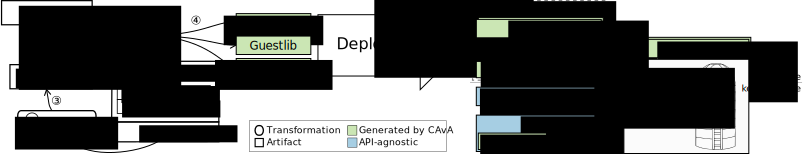
\includegraphics[width=0.5\linewidth]{figures/overview.png}
\caption{Data processed by two API stacks must pass through the guest application}
\label{fig:overview}
\end{figure}

Under a typical API-remoting system, applications that pipeline disparate accelerator frameworks are burdened with redundant data movement. All inter-accelerator data movement must take place in the guest application as that is where the accelerators are in the same logical address space. Figure~\ref{fig:overview} illustrates this scenario: when an API-1 function is invoked, associated data is copied from the guest application to executor-1, and then to device-1’s memory. Once the function finishes executing on device-1, the result is copied back to the guest VM. When a function from API-2 is invoked, the same data (i.e., the output of the API-1 function) is copied to executor-2 and then to device-2 to be processed.

In order to eliminate redundant data movement when an application uses multiple accelerators via API-remoting, the hypervisor must track the data passed to these API calls. The hypervisor must keep track of where the data flowed from and to, the validity of different copies of the data (e.g., if the data is modified on the accelerator, but hasn’t been copied back to the accelerator silo, or the guest application), and eliminate redundant data movement. As an example, if a guest application were to invoke the cudaMempyDtoH() function to copy data back from an Nvidia GPU, and then invoke the Intel QAT compression function cpaDCCompressData2() on the same data without modifying it in any way, the hypervisor should be able to detect this and elide the copying of data to and from the guest application.

vTask is an application-transparent data orchestration system that optimizes data movement among accelerators virtualized via API-remoting. vTask leverages information from API annotations (cite AvA) to track data buffers across the guest application, the executors servicing API calls made by the guest, and the accelerator hardware. vTask optimizes data movement across these components while ensuring that a coherent view of the data buffer is presented to anyone attempting to read the data. vTask requires no changes to the guest application or annotations of any kind from the application programmer; annotations provided to virtualize the API (by the device or virtualization vendor) are leveraged to infer semantics of the data buffers managed.

We prototyped vTask in AvA, a state-of-the-art para-virtual API-remoting system for KVM. vTask relies on device-side buffer allocation and deallocation API calls to determine buffer lifetime. vTask also leverages special annotations to explicitly specify buffer lifetime provided by LAPIS, AvA’s API description language. vTask implements a simple MESI-style coherence protocol to track spatial validity of data (i.e., to track where the latest data is present). vTask relies on optimizations such as shared memory, Unified Virtual Memory, and PCIe Peer-to-Peer (P2P) data transfer where available, but does not make assumptions about their universal availability.

vTask can handle data movement between both local and remote devices. When API-remoting to a remote system, the devices used by the guest application may be present on separate machines. vTask takes care to eliminate costly data transfers over the network by adhering to the principle of lazy loading wherever possible, i.e., data is not moved until a demand fault occurs.

Evaluating vTask on Y applications that different combinations of the ten accelerators supported by AvA shows that vTask improves performance by X\% on average when all devices are on the same machine, and Z\% when the devices are on remote hosts.

This work makes the following contributions:
\begin{itemize}[nosep,leftmargin=1em,labelwidth=*,align=left]
\item We identify and measure performance problems with using multiple accelerators via API-remoting
\item We propose an application-transparent data orchestration framework, vTask, which transparently manages data buffers in the hypervisor and elides redundant data movement.
\item We prototyped vTask in AvA with support for both local and remote accelerators, and used it to evaluate the performance of applications that use different combinations of the ten accelerators supported by AvA. vTask improves application performance by XX% on average.
\end{itemize}
% -*- fill-column: 85; -*-
%!TEX root = ../dissertation.tex
\section{Related Work}
\label{s:related}

Chapter~\ref{sec:related} provides detailed related work; this section
addresses related work not covered there. Our previous work~\cite{hotos-ava}
proposed many key ideas in \model; this paper fleshes out and evaluates those
ideas.

\paragraphbe{FPGA virtualization}
has a long history~\cite{codezero,plessl2005zippy,
score,tartan06asplos,virtualRC,huang09fpgavirt,brant2012zuma,rcmw,
intermediate-fabrics}. Most prior work relies on hardware-specific features,
focuses on sharing in a single protection domain~\cite{amorphos}, or
virtualization primitives~\cite{cascade}. \model can be combined with any of
these techniques to virtualize FPGA accelerators.

\paragraphbe{Nooks}~\cite{nooks} uses kernel-level interposition
mechanisms that are similar in spirit to \Model. \Model's compiler generates
components that, like the wrappers and XPC in Nooks, provide transparent
control across address space and machine boundaries. Object tracking and
shadow copies in Nooks' \emph{NIM} are similar to the object tracking and
shadow buffers in \model.

\paragraphbe{RPC frameworks}~\cite{grpc,thrift,corba,Yang1996} provide an
interface description language (IDL) and tools to easily implement those
interfaces. Unlike the \compiler language, these IDLs do not capture all the
semantics of \emph{existing} C interfaces required to implement a \novtechabbrv
API remoting design. \Compiler also generates code for controlling remote
resources.

\paragraphbe{Program specification languages}~\cite{mssal} allow programmers
to specify properties of functions and their behavior, and are generally used
to check correctness, either statically (e.g., with model checking) or
dynamically (e.g., by inserting checks in the program). While such languages
allow (nearly) arbitrary predicates on programs, they are not designed to
provide semantic information to other tools, In addition, these languages are
not designed to specify how API calls are performed, and do not support
features like state tracking. \Speclang is optimized to allow easy and
specific descriptions of APIs and how calls should be performed.

\paragraphbe{Foreign Function Interface} tools allow one language to call
functions written in another, such as C.
Some~\cite{swig} make use of C headers, but require manual annotations in many
common cases. Unlike \model, language specific DSLs~\cite{cython,jna},
do not support marshalling data structures and encapsulate rather than export
the C API.
Cross-language serialization standards and frameworks~\cite{protobuf, msgpack,
ecma404}, only provide serialization for a set of primitives and supported
constructs. The user must write code to translate their data structure into
the language of the framework and provide their own transport for the
serialized data.

% % Appendices
% \appendix

% % Switch to 1" title margins for appendices
% \titlespacing{\chapter}{0in}{-.38in}{11pt}

% % Appendix 1
% \input{ap1}

% References
\clearpage
\phantomsection

{
\def\chapter*#1{} % suppress bibliograph header.
\begin{singlespace}
\addcontentsline{toc}{chapter}{BIBLIOGRAPHY}
\begin{center}
\normalfont \textbf{BIBLIOGRAPHY}
\vspace{17pt}
\end{center}

\bibliographystyle{plain}
\bibliography{ref}
\end{singlespace}
}

\end{document}